\documentclass[a4paper,11pt]{article} %openright - los capítulos empiezan en páginas impares; 10pt tamaño de texto
\usepackage[spanish]{babel}
\usepackage[utf8]{inputenc} %para trabajar con símbolos no anglosajones

\usepackage[title,titletoc,toc]{appendix}
\usepackage{textcomp}
\usepackage{graphicx}
\usepackage{eso-pic}
\usepackage{transparent}
\usepackage{enumerate}
\usepackage{fancyhdr}
\usepackage{graphicx}
\usepackage{subfigure}
\usepackage{float}
\usepackage{colortbl}
\usepackage{amsmath}
\usepackage{gensymb}
\usepackage{multirow}
\usepackage{subfigure}
\usepackage{minted}
\usepackage{anysize}
\usepackage{fontawesome}

%
% Hace una marca de agua
%

%\usepackage{background}
%\SetBgContents{ENTREGA PROVISIONAL}
%\SetBgScale{5} %% Escala del texto
%\SetBgColor{black!10!white} %% Tonalidad



\marginsize{3cm}{2cm}{2cm}{2cm} % Controla los márgenes {izquierda}{derecha}{arriba}{abajo}. 

\graphicspath{{Pictures/}} %path de los gráficos

%
% A continuación se define la portada
%

\newcommand\BackgroundPic{%
	\put(0,0){%
		\parbox[b][\paperheight]{\paperwidth}{%
			\vfill
			\centering
			
\includegraphics[width=\paperwidth,height=\paperheight,%
			keepaspectratio]{PortadaAzul.pdf}%
			\vfill
		}}}
%
% A continuación está el encabezado y pie de página
%
		
\pagestyle{fancy}
\fancyfoot[RE,RO]{Página \thepage}
\fancyfoot[C]{\ }
\fancyfoot[LE,LO]{\textcolor{gray}{SED. Proyecto Ascensor}}
\fancyhead[RE,RO]{Grupo N\textdegree 4}
\fancyhead[LE,LO]{\ }

%
% A continuación empieza el documento
%

\begin{document}

    
    %
    % A continuación empieza la portada del documento
    %

	\begin{titlepage}
		\pagestyle{empty}
		\AddToShipoutPicture*{\BackgroundPic}
		\begin{center}
			\Huge \textbf{Proyecto final de asignatura:\\ \textsc{“Ascensor”}}
			\vspace{5cm}
			
			\Large \textsc{Dpto. Electrónica, Automática e Informática	Industrial} \\ 
			
			\large \textsc{ETSIDI - UPM}
		\end{center}
		\vspace{8cm}
		
		\hspace{1cm}\large Asignatura de Sistemas Electrónicos Digitales
		
		\hspace{1cm}\large Curso 2016-2017\\
		
		
		\hspace{1cm}\large \textbf{Arancha Canelo Martin} \hspace{1.65cm} N\textdegree 50654 \\ 
		
		\hspace{1cm}\large \textbf{Enrique Heredia Aguado} \hspace{1.4cm} N\textdegree 50688 \\ 
		
		\hspace{1cm}\large \textbf{Alberto Beneit Benita} \hspace{1.95cm} N\textdegree 51104
		\ClearShipoutPicture
		\thispagestyle{empty}
	\end{titlepage}
	
	\pagestyle{fancy}
	
	%\addtocontents{toc}{\hspace{-7.5mm} \textbf{Contenidos:}}
	\addtocontents{toc}{\hfill \textbf{Página:} \par}
	\addtocontents{toc}{\vspace{-2mm} \hspace{-7.5mm} \hrule \par}
	\tableofcontents
	\newpage

    %
    % A continuación empieza el contenido del documento
    %
    \section{Introducción:} \label{section:Introduccion}
        

\subsection{Objetivos:}
    \begin{itemize}
        \item Diseño de la lógica de control de un ascensor.
        \item Implementación y validación de dicho diseño en lenguaje VHDL.
        \item Simulación de cada entidad implementada para verificar su funcionamiento mediante un testbench en código VHDL.
        \item Sintetizado sobre la tarjeta SPARTAN-3 Starter Kit del laboratorio
    \end{itemize}
    
\subsection{Funcionamiento general del Ascensor y requisitos:}

   El trabajo consiste en diseñar el controlador de un ascensor único en una vivienda.
    \begin{itemize}
        \item Requisitos mínimos:
        \begin{itemize}
    		    \item El ascensor debe tener un mínimo de 4 pisos.
    		    \item Las entradas al circuito serán, por un lado, el piso al que el usuario desea ir y el piso en el que está el ascensor en un momento dado.
    		    \item Hay 2 salidas, la del motor (2 bits) y la de la puerta (1 bit).
    		    \item El ascensor debe ir al piso indicado, cuando llegue abrirá las puertas que permanecerán así hasta que se reciba otra llamada.
    		    \item Si mientras que el ascensor se mueve, se pulsan otros botones no se debe hacer caso.
    		    \item Utilizar los LEDs y los Displays para visualizar la información.
    	\end{itemize}
        \item Funcionalidad extra
        \begin{itemize}
            \item [1-] Añadimos dos salidas. 
            \begin{itemize}
        		    \item Piso al que el usuario desea ir.
                \item Piso en el que está el ascensor.
            \end{itemize}  
            Mostrando ambas por dos dígitos distintos del Display.
            \item [2-] Aumentamos el número de pisos que puede almacenar simultáneamente el programa a tres, debe ir a cada uno de ellos en el mismo orden que fueron introducidos.
            \begin{itemize}
        		    \item Se muestran todos los pisos almacenados.
      	  	    \item Se mueva o no el ascensor, se hace caso de los botones pulsados mientras alguna de las tres variables esté "vacía".
    	    \end{itemize}
	    \end{itemize}
        \item Puertos usados:
        \begin{itemize}
     	   	\item Pulsadores de la FPGA, se usan para la entrada del piso en el que está el ascensor en un momento dado, representan finales de carrera (uno por planta).
    		    \item Cuatro Interruptores, empleados para introducir el piso al que el usuario desea ir, representan los botones del ascensor (uno por planta).
    		    \item Cuatro dígitos del Display, dedicados a mostrar el estado del motor, el estado de la puerta el piso en el que está el ascensor y el piso al que va el ascensor.
    		    \item LEDs de la FPGA, utilizados para representar los dos pisos almacenados a los que posteriormente debe ir el ascensor.
    	\end{itemize}
	\end{itemize}

\subsection{Placa Spartan-3 Starter Kit Board} \label{subsection:Spartan-3}
    
    Para la implementación de este proyecto y si realización sobre un soporte físico real se utilizará la placa Spartan-3 Starter Kit Board de Xilinx, que incluye la FPGA así como otros componentes que nos vendrán bien a la hora de simular el comportamiento del ascensor.

    En las figuras que se muestran a continuación se pueden ver la distribución de los componentes del Kit:

    \begin{figure}[H]
            \centering
            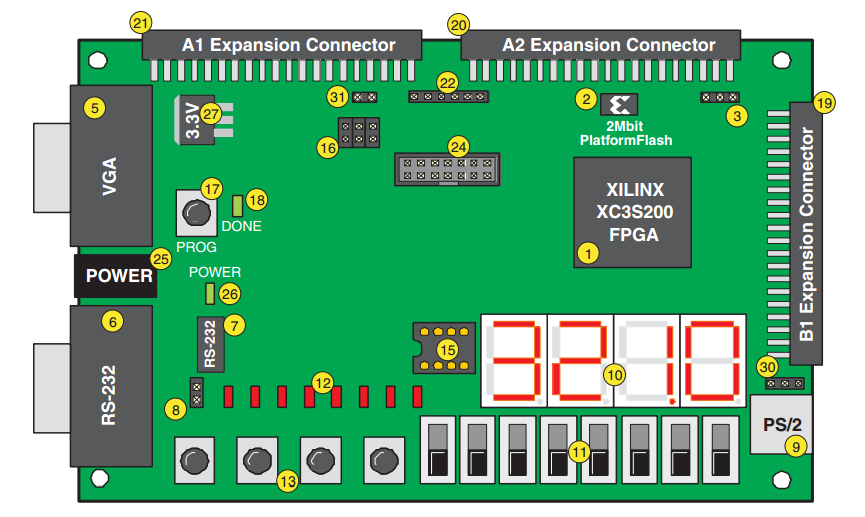
\includegraphics[width = 0.8\textwidth ]{Spartan3TopSide}
            \caption{Placa Spartan-3 (parte superior)}
            \label{fig:Spartan3TopSide}
    \end{figure}

    \begin{figure}[H]
            \centering
            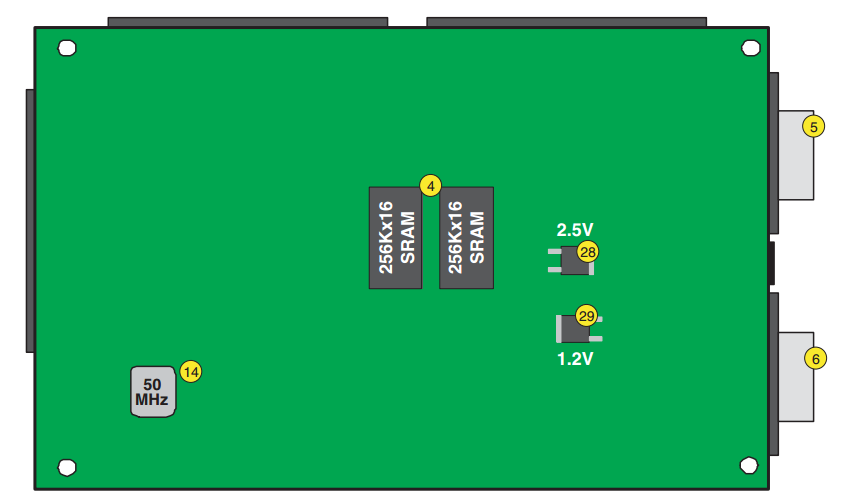
\includegraphics[width = 0.8\textwidth ]{Spartan3BottomSide}
            \caption{Placa Spartan-3 (parte inferior)}
            \label{fig:Spartan3BottomSide}
    \end{figure}

    Nos centraremos en los componentes más importantes que utilizaresmos para la realización de este proyecto:

    \begin{itemize}
        \item [1.] Xilinx Spartan-3 XC3S200 FPGA  (encapsulado XC3S200FT256). Compuesta por 200000 puertas.
        \item [2.] 2Mbit Xilinx XCF02S Platform Flash.
        \item [4.] 1M-byte of Fast Asynchronous SRAM.
        \item [10.] Cuatro displays LED de 7 segmentos.
        \item [11.] Ocho interruptores.
        %\item [12.] Ocho salidas LED independientes.
        \item [13.] Cuatro pulsadores.
        \item [14.] Cristal osculador (CLK) de 50MHz.
        \item [18.] LED indicador de que la FPGA ha sido configurada correctamente

    \end{itemize}

    Las salidas físicas para los \textbf{displays de 7 segmentos} se encuentran en los pines que se pueden ver en la siguiente tabla. Los displays se encuentran representados con el número 10 en la figura (\ref{fig:Spartan3TopSide}) del apartado (\ref{subsection:Spartan-3}). \\ 

    Como se puede ver en la figura los 4 displays comparten 8 pines de control, para elegir un display u otro están los Ánodos de control, en la tabla (\ref{tab:anodoControl}). \\ 

    Es importante tener en cuenta que los cuatro display de 7 segmentos comparten la entrada de 7 bits que codifica el caracter; se elige por que display se muestra dicha información sacando un valor de alto nivel por el ánodo de control correspondiente. \\ 

    \begin{table}[H]
            \centering
            \begin{tabular}{|c|c|c|c|c|c|c|c|c|}
                \hline
                \rowcolor[rgb]{0.21,0.69,0.87}\multicolumn{9}{|c|}{  \textbf{ {Salidas físicas Display 7 segmentos}}} \\
                \hline \hline
                \textbf{  Segmento  } & A & B & C & D & E & F & G & DP \\ 
                \hline
                \textbf{  FPGA Pin  }  & E14 & G13 & N15 & P15 & R16 & F13 & N16 & P16 \\ 
                \hline
                \multicolumn{9}{|c|}{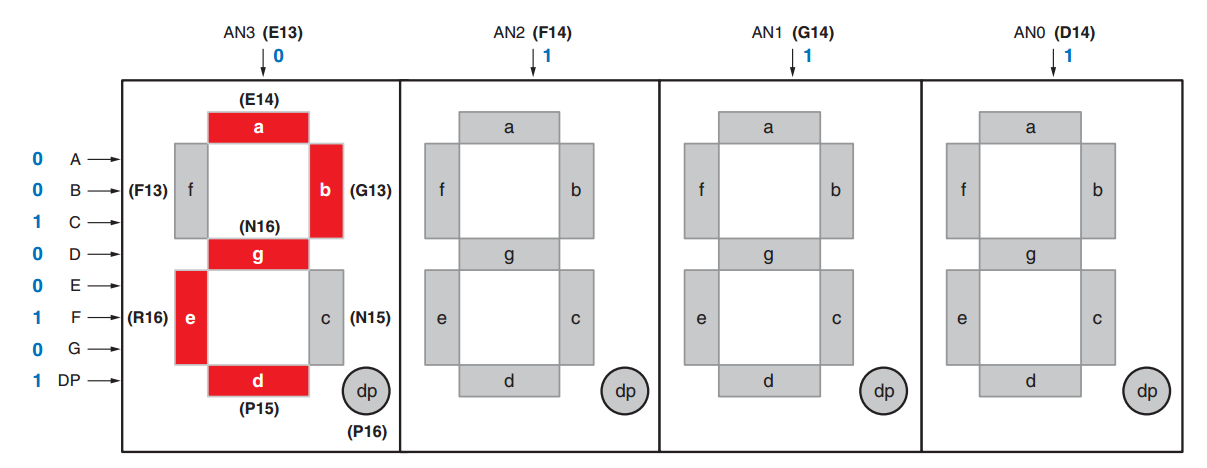
\includegraphics[width = 0.8\textwidth ]{Spartan3-7segment}}\\
                \hline
                 
            \end{tabular}
        \caption{ Salidas físicas de los displays en la Spartan-3 }
        \label{tab:tablaSalidas7Segmentos}
    \end{table}

    \begin{table}[H]
            \centering
            \begin{tabular}{|c|c|c|c|c|}
                \hline
                \rowcolor[rgb]{0.21,0.69,0.87}\multicolumn{5}{|c|}{  \textbf{ {Ánodos de control}}} \\
                \hline \hline
                \textbf{  Anodo Control  } & AN3 & AN2 & AN1 & AN0  \\
                \hline
                \textbf{  FPGA Pin  } & E13 & F14 & G14 & D14  \\
                \hline
                 
            \end{tabular}
        \caption{ Ánodos control (activos a nivel bajo) para los display de 7 segmentos }
        \label{tab:anodoControl}
    \end{table}

    Las entradas correspondientes a los \textbf{interruptores} se pueden ver en la siguiente tabla. Estos interruptores se encuentran representados con el número 11 en la figura (\ref{fig:Spartan3TopSide}) del apartado (\ref{subsection:Spartan-3}).

    \begin{table}[H]
            \centering
            \begin{tabular}{|c|c|c|c|c|c|c|c|c|}
                \hline
                \rowcolor[rgb]{0.21,0.69,0.87}\multicolumn{9}{|c|}{  \textbf{ {Entradas Interruptores}}} \\
                \hline \hline
                \textbf{  Interruptor  } & SW7 & SW6 & SW5 & SW4 & SW3 & SW2 & SW1 & SW0 \\
                \hline
                \textbf{  FPGA Pin  } & K13 & K14 & J13 & J14 & H13 & H14 & G12 & F12 \\
                \hline
                 
            \end{tabular}
        \caption{ Entradas físicas de los interruptores en la Spartan-3 }
        \label{tab:tablaEntradasInterruptores}
    \end{table}

    Los pines de entrada correspondientes a los \textbf{pulsadores} se pueden ver en la siguiente tabla. Estos componentes se corresponden con los representados con el número 13 en la figura (\ref{fig:Spartan3TopSide}) del apartado (\ref{subsection:Spartan-3}).

    \begin{table}[H]
            \centering
            \begin{tabular}{|c|c|c|c|c|}
                \hline
                \rowcolor[rgb]{0.21,0.69,0.87}\multicolumn{5}{|c|}{  \textbf{ {Entradas Pulsadores}}} \\
                \hline \hline
                \textbf{  Pulsador  } & BTN3 (Reset) & BTN2 & BTN1 & BTN0  \\
                \hline
                \textbf{  FPGA Pin  } & L14 & L13 & M14 & M13  \\
                \hline
                 
            \end{tabular}
        \caption{ Entradas físicas de los pulsadores en la Spartan-3 }
        \label{tab:tablaEntradasPulsadores}
    \end{table}

%    Por ahora no utilizamos los LEDs, queda comentado por si volvemos a usarlos.
%
%    Como se ha dicho en el apartado (\ref{subsection:Spartan-3}) la placa incorpora ocho LEDs, representados con el número 12 en la figura (\ref{fig:Spartan3TopSide}). A continuación se muestra la correlación de cada LED con la patilla de la FPGA:

%   \begin{table}[H]
%            \centering
%            \begin{tabular}{|c|c|c|c|c|c|c|c|c|}
%                \hline
%                \rowcolor[rgb]{0.21,0.69,0.87}\multicolumn{9}{|c|}{  \textbf{ {Salidas LED}}} \\
%                \hline \hline
%                \textbf{  LED  } & LD7 & LD6 & LD5 & LD4 & LD3 & LD2 & LD1 & LD0 \\
%                \hline
%                \textbf{  FPGA Pin  } & P11 & P12 & N12 & P13 & N14 & L12 & P14 & K12  \\
%                \hline
%                 
%            \end{tabular}
%        \caption{ Salidas físicas de los LEDs en la Spartan-3 }
%        \label{tab:tablaSalidasLED}
%    \end{table}

\subsection{Estructura de la memoria e información útil}

    En los siguientes apartados de la memoria se puede encontrar la explicación detallada del funcionamiento y codificación de la lógica del ascensor descrito, concretamente:
    \begin{itemize}
        \item Apartado \ref{section:DiagBloques}: Se detalla el funcionamiento interno de cada entidad o arquitectura así como su interfaz. A su vez se describe la relación entre las diferentes entidades
        \item Apartado \ref{section:Codigo}: Se adjunta la programación de cada entidad o arquitectura así como su correspondiente testbech.
        \item Apartado \ref{section:PruebasYResultados}: Se comentan los aspectos prácticos de como se ha cargado esta información en la FPGA así como los resultados obtenidos.
        \item Apéndice \ref{app:codEntSal}: Se adjuntan las tablas donde se especifica la codificación que se ha utilizado para el funcionamiento interno del ascensor.
    \end{itemize}
    
    Todo el proyecto, tanto el documento en código \LaTeX\  como los ficheros VHDL se pueden encontrar en Github \faGithub\ en el siguiente enlace: https://github.com/enheragu/Elevator-VHDL
 %importa el fichero IntroObj.tex con la introducción, objetivos y explicación general del proyecto
        
    \section{Diagrama de bloques:} \label{section:DiagBloques}
    
        \subsection{Bloque \textit{Acensor}:}
    
    La interfaz, entradas y salidas, de este bloque se puede ver su representación en la Figura \ref{fig:BloqueIAscensor}:
    
    \begin{figure}[H]
		    \centering
		    \includegraphics[width = 0.8\textwidth ]{BloqueAscensor}
		    \caption{Diagrama Interfaz Bloque PisoActual}
		    \label{fig:BloqueIAscensor}
	\end{figure}
	
	Esta es una entidad de alto nivel que encapsula todo el funcionamiento del ascensor. Se puede ver el diagrama de bloques interno de esta entidad en la siguiente figura: 
	
	\begin{figure}[H]
		    \centering
		    \includegraphics[width = 1\textwidth ]{BloqueAscensorInterior}
		    \caption{Diagrama interno del Bloque PisoActual}
		    \label{fig:BloqueIAscensorInterior}
	\end{figure}
	
	Cada bloque se desgrana en los siguientes apartados.
	

\subsection{Bloque \textit{Controlador Motor}:}

\subsection{Bloque \textit{Controlador Puerta}:}

\subsection{Bloque \textit{Decodificador a 7 segmentos}:}
    Este bloque es el encargado de traducir el piso en el que se encuentra el ascensor y el piso objetivo para poder mostrarlo en el display de 7 segmentos. Para ello es importante recordar el Cuadro (\ref{tab:tabla1ApendiceA}) del Apéndice \ref{app:codEntSal} donde podemos ver como se codifica internamente el número de piso. \\ 
    
    La salida que se verá en el display para cada caso se puede ver en la figura siguiente:
    
    \begin{figure}[H]
		    \centering
		    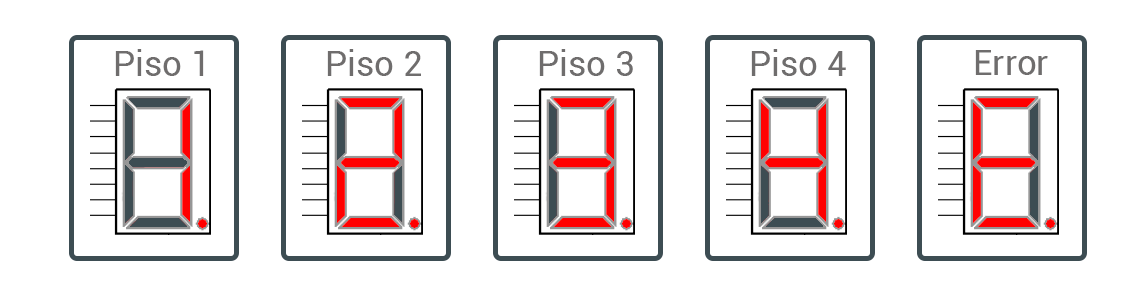
\includegraphics[width = 1\textwidth ]{displays7s}
		    \caption{Salida en los displays de 7 segmentos}
		    \label{fig:displays7s}
	\end{figure}
    
    La interfaz, entradas y salidas, de este bloque se puede ver su representación en la Figura \ref{fig:BloqueDecodificador7seg}:
    
    \begin{figure}[H]
		    \centering
		    \includegraphics[width = 0.7\textwidth ]{BloqueDecodificador}
		    \caption{Diagrama Interfaz Bloque Decodificador a 7 segmentos}
		    \label{fig:BloqueDecodificador7seg}
	\end{figure}
\subsection{Bloque \textit{Divisor de frecuencia}:}

\subsection{Bloque \textit{PistoActual}:}
    Como se ha dicho anteriormente en cada piso hay un final de carrera que detecta el paso del ascensor. El prpósito de este bloque es el de filtrar dicha entrada de 4 bits. En este caso lo que interesa es saber en que piso estoy o en que piso he estado por última vez. Cuando el ascensor se encuentra entre dos pisos la entrada de los sensores será \textit{0000}, este bloque lo que hará será mantener en la salida del mismo el último piso por el que haya pasado el ascensor. \\ 
    
    Como se puede apreciar en el siguiente diagrama este bloque tiene una entrada, un vector de 4 bits (los finales de carrera de cada piso) y una salida, también de 4 bits, codificando el piso en el que se encuentra actualmente. \\ 
    
    Se puede consultar dicha codificación en el Cuadro (\ref{tab:tabla1ApendiceA}) del Apéndice \ref{app:codEntSal}. \\ 
    
    La interfaz, entradas y salidas, de este bloque se puede ver su representación en la Figura \ref{fig:BloquePisoActual}:
    
    \begin{figure}[H]
		    \centering
		    \hspace*{-1.8cm}
		    \includegraphics[width = 0.6\textwidth ]{BloquePisoActual}
		    \caption{Diagrama Bloque PisoActual}
		    \label{fig:BloquePisoActual}
	\end{figure}
	
	Se puede consultar el código VHDL de este módulo en el Apartado \ref{code:PisoActual} así como el código de su testbench correspondiente en el Apartado \ref{code:PisoActual_tb}.

\subsection{Bloque \textit{Bloqueador pisoVoy}:}
    
    La interfaz, entradas y salidas, de este bloque se puede ver su representación en la Figura \ref{fig:BloqueBloqueadorPisoVoy}:
    
    
    \begin{figure}[H]
		    \centering
		    \hspace*{-1.8cm}
		    \includegraphics[width = 0.6\textwidth ]{BloqueBloqueadorPisoVoy}
		    \caption{Diagrama Bloque Bloqueador PisoVoy}
		    \label{fig:BloqueBloqueadorPisoVoy}
	\end{figure}
	

\subsection{Bloque \textit{Comparador}:}

    La interfaz, entradas y salidas, de este bloque se puede ver su representación en la Figura \ref{fig:BloqueComparador}:
    
    \begin{figure}[H]
		    \centering
		    \includegraphics[width = 0.6\textwidth ]{BloqueComparador}
		    \caption{Diagrama Bloque Comparador}
		    \label{fig:BloqueComparador}
	\end{figure} %importa el fichero DiagramaBloques.tex
        
    \section{Código:} \label{section:Codigo}
    
        \subsection{Código Bloque \textit{Decodificador a 7 segmentos}:} \label{code:Decodificador7s}
	Como se a adelantado en la sección (\ref{bloque:Decodificador7s}) este bloque es el encargado de adaptar las señales de salida a los displays. Para ello se asigna a cada posible entrada (cada piso) con una señal de salida que codifica en los 7 segmentos el caracter deseado, incluyendo un caracter de error.

	\inputminted[frame=lines,fontsize=\footnotesize,linenos]{vhdl}{CodeFiles/Decodificador7s.vhd}
	
	Como se puede ver en la Figura (\ref{fig:BloqueDecodificador7sOK}) el esquema obtenido una vez programado y sintetizado se corresponde con el que se pretendía.
    \begin{figure}[H]
		    \centering
		    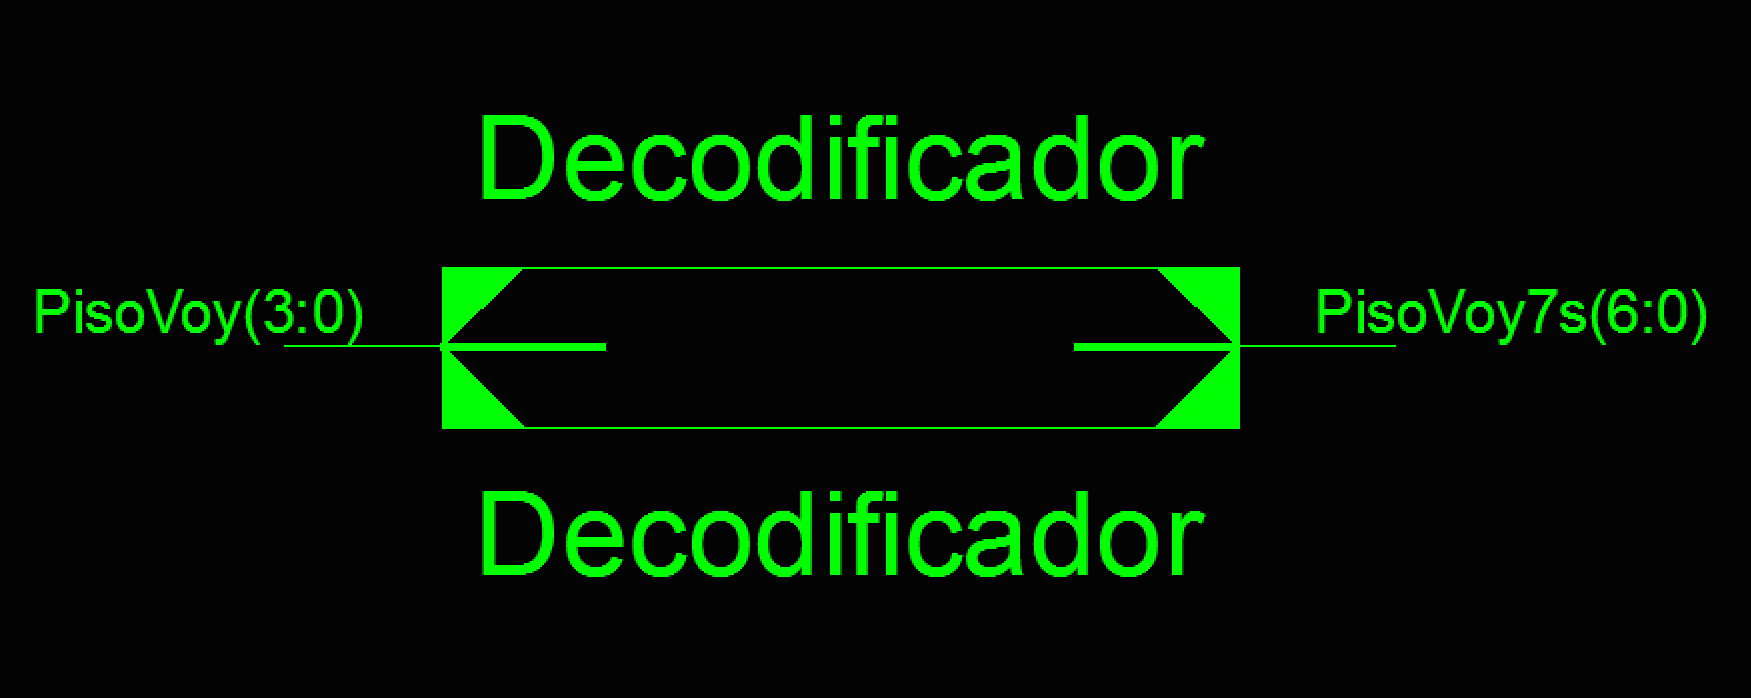
\includegraphics[width = 0.6\textwidth ]{BloqueDecodificador7sOK}
		    \caption{Esquema exterior del bloque Decodificador7s}
		    \label{fig:BloqueDecodificador7sOK}
	\end{figure}
    Además podemos ver en la Figura (\ref{fig:BloqueDecodificador7sImplementacion}) como se compone internamente el bloque, como se codifica en hardware esta utilidad:
    \begin{figure}[H]
		    \centering
		    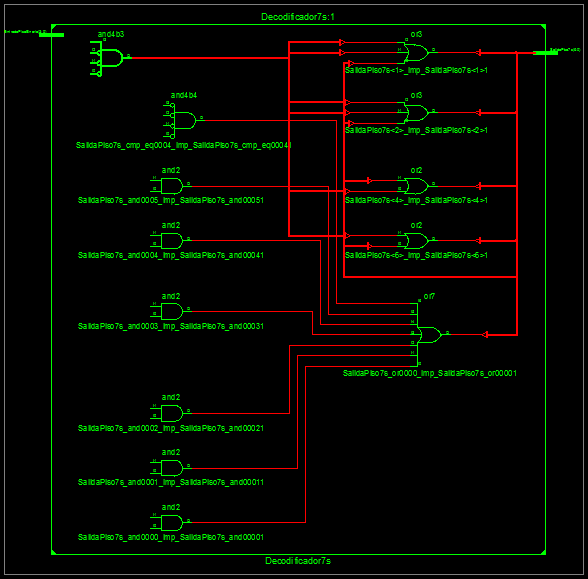
\includegraphics[width = 0.9\textwidth ]{BloqueDecodificador7sImplementacion}
		    \caption{Esquema interno del bloque Decodificador7s}
		    \label{fig:BloqueDecodificador7sImplementacion}
	\end{figure}

\subsection{Código Bloque \textit{Decodificador a 7 segmentos (testbench)}:} \label{code:Decodificador7s_tb}
	
	\inputminted[frame=lines,fontsize=\footnotesize,linenos]{vhdl}{CodeFiles/Decodificador7s_tb.vhd}
	
	Utilizando este testbench se obtiene el comportamiento que se puede ver en la Figura (\ref{fig:SimulacionDecodificador7s}):

    \begin{figure}[H]
		    \centering
		    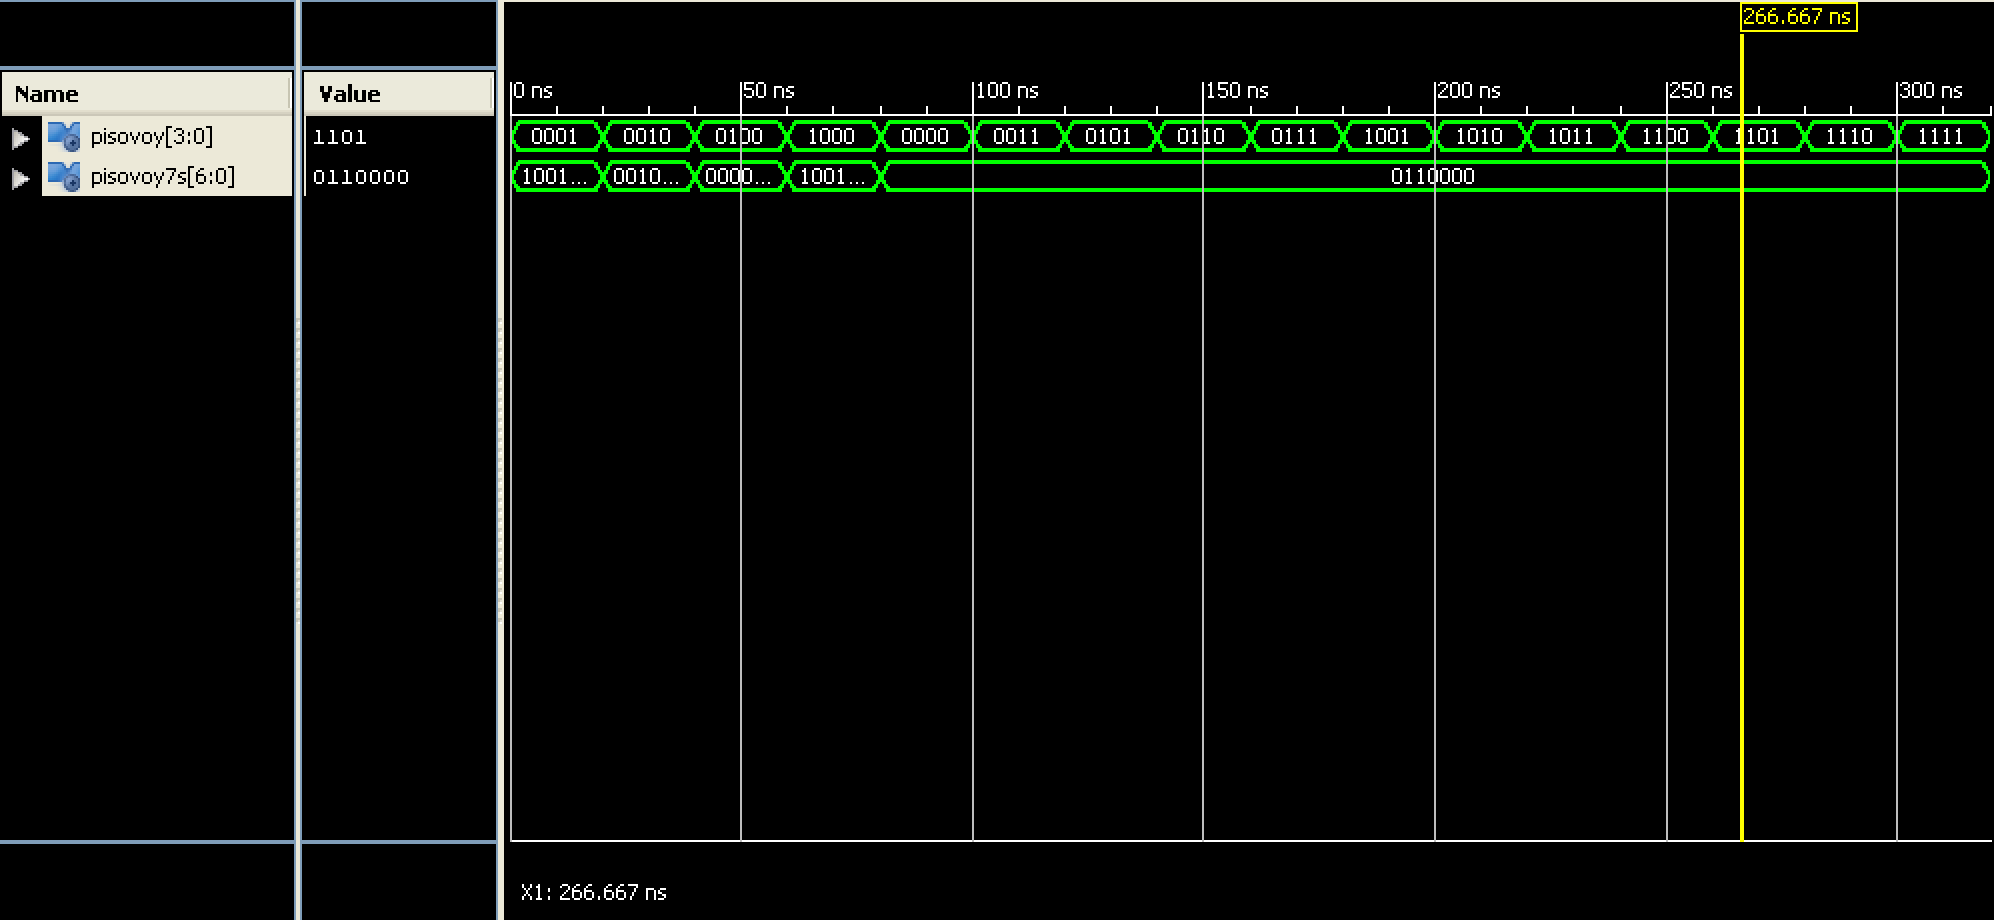
\includegraphics[width = 0.8\textwidth ]{SimulacionDecodificador7s}
		    \caption{Simulación del testbench del bloque Decodificador7s}
		    \label{fig:SimulacionDecodificador7s}
	\end{figure}

\subsection{Código Bloque \textit{Divisor de frecuencia}:} \label{code:DivisorFrecuencia}
	Como se ha visto en la seccción (\ref{subsection:Spartan-3}) los cuatro displays comparten la salida de 7 bits, cambiando de un display a otro a través de los ánodos de contro. En este bloque se va alternando de un ánodo a otro para mostrar por cada display la salida correspondiente sin que se pise la información y a una frecuencia suficiente para que el parpadeo no sea apreciable. A continuación se puede ver el código que codifica esta funcionalidad: \\ 

	\inputminted[frame=lines,fontsize=\footnotesize,linenos]{vhdl}{CodeFiles/DivisorFrecuencia.vhd}

\subsection{Código Bloque \textit{Divisor de frecuencia (testbench)}:} \label{code:DivisorFrecuencia_Tb}
	\inputminted[frame=lines,fontsize=\footnotesize,linenos]{vhdl}{CodeFiles/DivisorFrecuencia_tb.vhd}

\subsection{Código Bloque \textit{PistoActual}:} \label{code:PisoActual}
	Como se ha explicado en la sección (\ref{bloque:PisoActual}) este bloque filtrará posibles lecturas que no nos interese pasar al comparador. De esta forma solo tomará como válidas los vectores que se correspondan con ela codificación de cada piso. Cuando entre una lectura que no se corresponde con ello se pasará el último piso detectado. Esta situación incluye cuando el ascensor de encuentra entre dos pisos (SensorEstoy = 0000) o posibles errores incoherentes que puedan darse debido a la electrónica como podría ser una lectura con valores "0110" o similar. A continuación se puede ver el código que codifica dichas funcionalidades: \\ 

    \inputminted[frame=lines,fontsize=\footnotesize,linenos]{vhdl}{CodeFiles/PisoActual.vhd}
    
    Como se puede ver en la Figura (\ref{fig:BloquePisoActualOK}) el esquema obtenido una vez programado y sintetizado se corresponde con el que se pretendía.
    \begin{figure}[H]
		    \centering
		    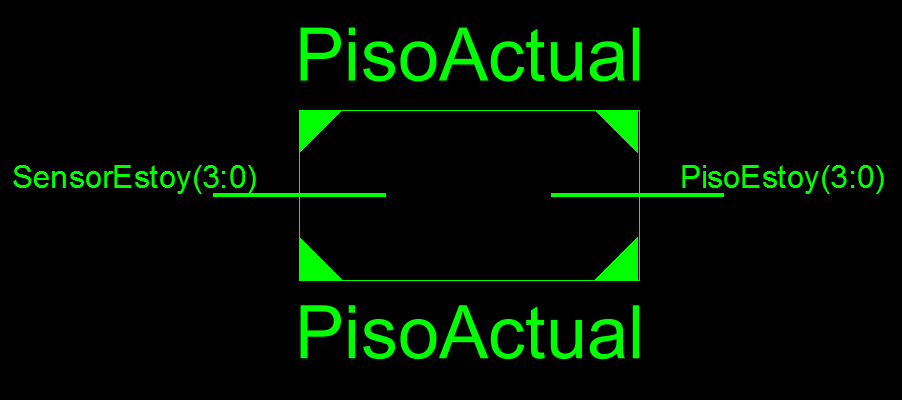
\includegraphics[width = 0.6\textwidth ]{BloquePisoActualOK}
		    \caption{Esquema exterior del bloque Piso Actual}
		    \label{fig:BloquePisoActualOK}
	\end{figure}
    Además podemos ver en la Figura (\ref{fig:BloquePisoActualImplementacion}) como se compone internamente el bloque, como se codifica en hardware esta utilidad:
    \begin{figure}[H]
		    \centering
		    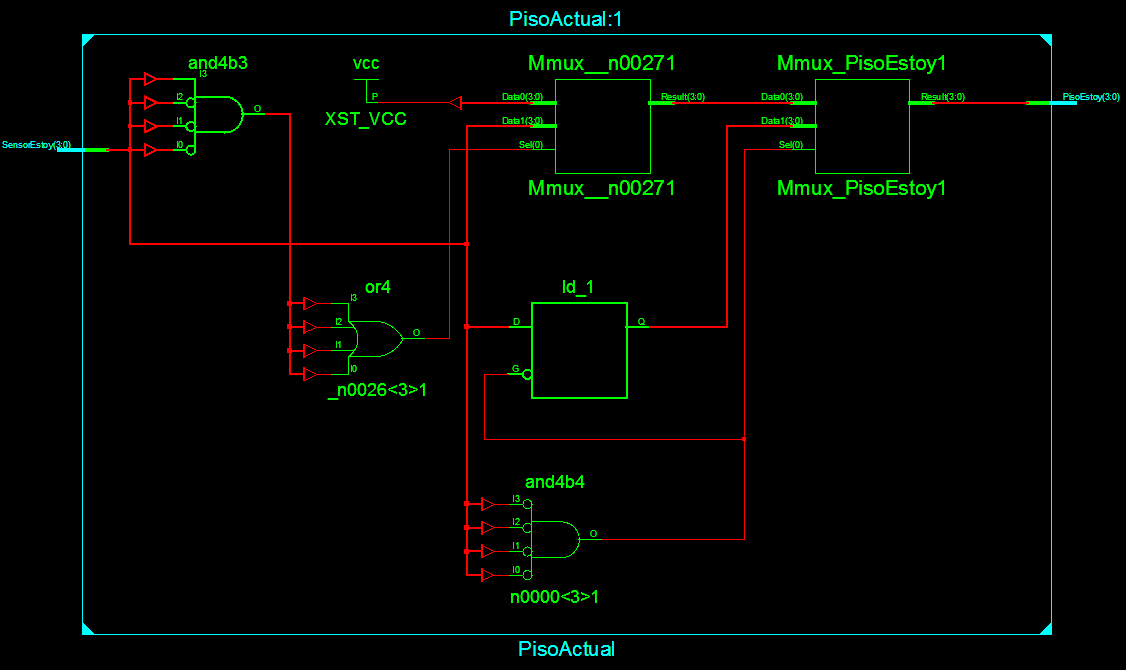
\includegraphics[width = 0.9\textwidth ]{BloquePisoActualImplementacion}
		    \caption{Esquema interno del bloque Piso Actual}
		    \label{fig:BloquePisoActualImplementacion}
	\end{figure}

\subsection{Código Bloque \textit{PistoActual (testbench)}:} \label{code:PisoActual_tb}
    \inputminted[frame=lines,fontsize=\footnotesize,linenos]{vhdl}{CodeFiles/PisoActual_tb.vhd}
    
    Utilizando este testbench se obtiene el comportamiento que se puede ver en la Figura (\ref{fig:SimulacionPisoActual}):

    \begin{figure}[H]
		    \centering
		    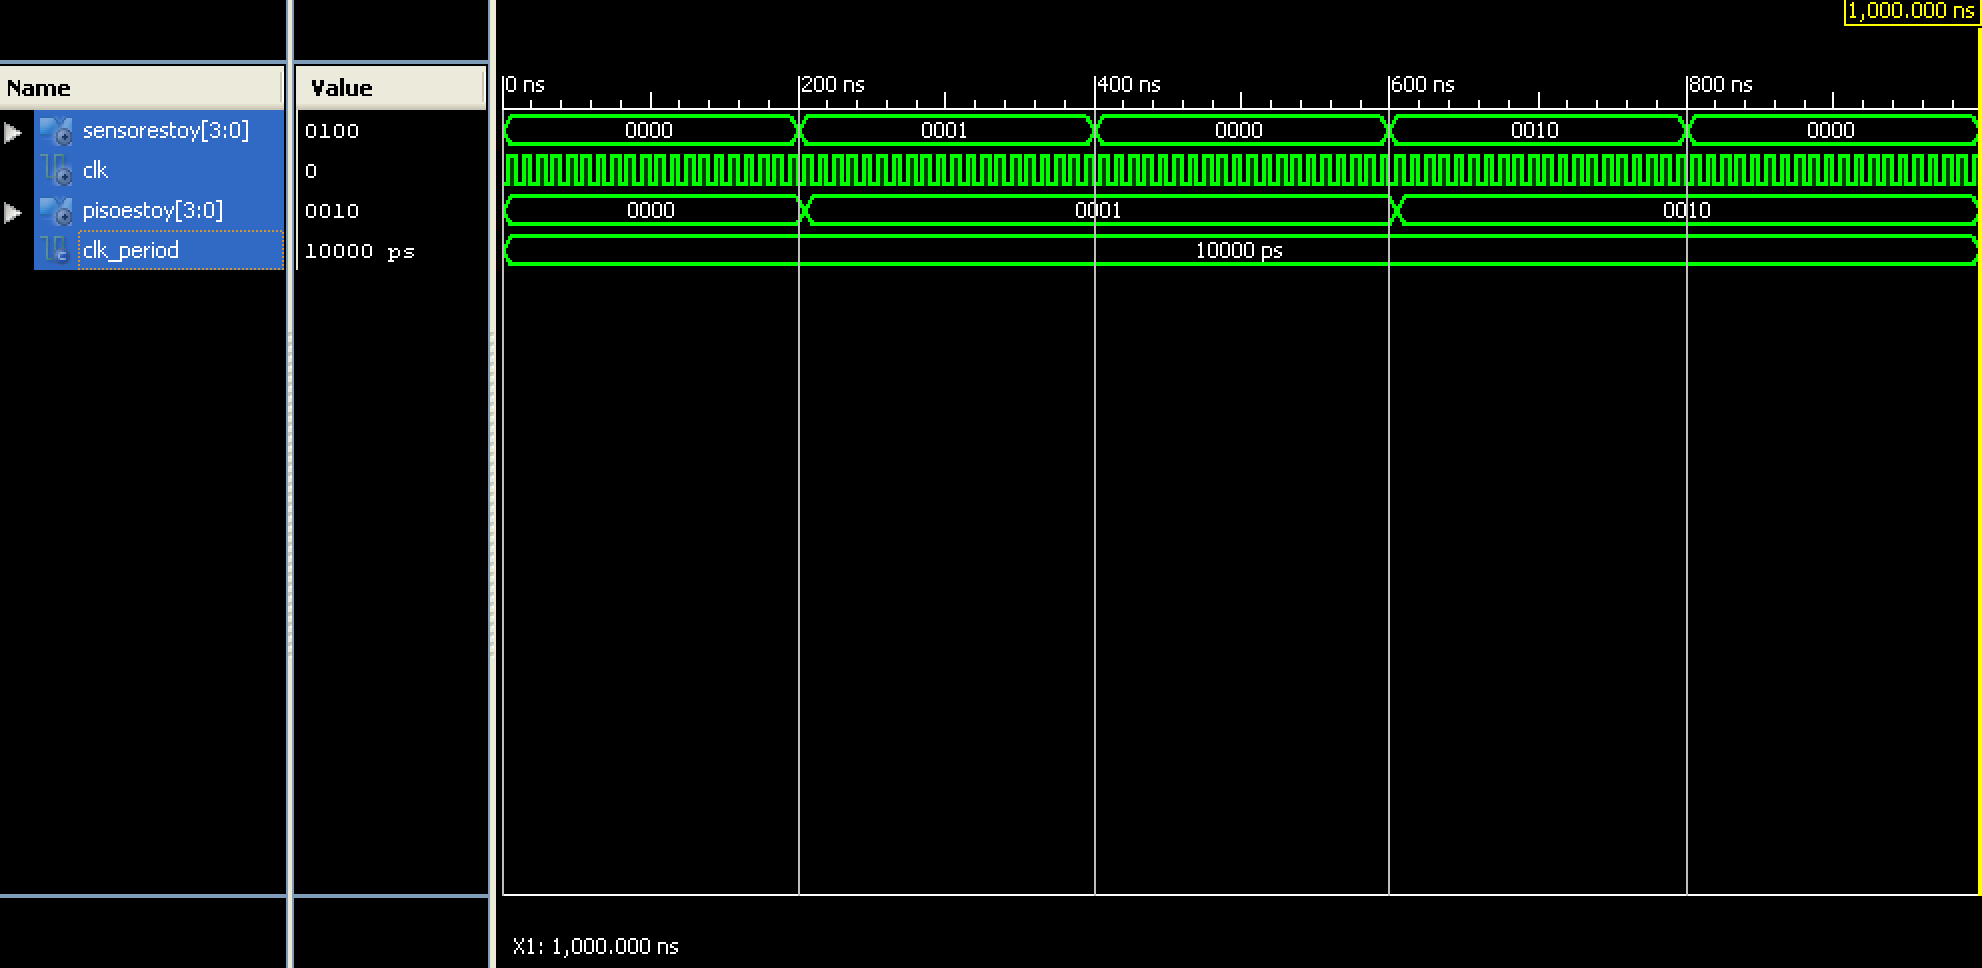
\includegraphics[width = 0.8\textwidth ]{SimulacionPisoActual}
		    \caption{Simulación del testbench del bloque PisoActual}
		    \label{fig:SimulacionPisoActual}
	\end{figure}


\subsection{Código Bloque \textit{Bloqueador PisoVoy}:} \label{code:BloqueadorpisoVoy}	
    \inputminted[frame=lines,fontsize=\footnotesize,linenos]{vhdl}{CodeFiles/BloqueadorPisoVoy.vhd}
	Como se puede ver en la Figura (\ref{fig:BloqueBloqueadorPisoVoyOK}) el esquema obtenido una vez programado y sintetizado se corresponde con el que se pretendía.
    \begin{figure}[H]
		    \centering
		    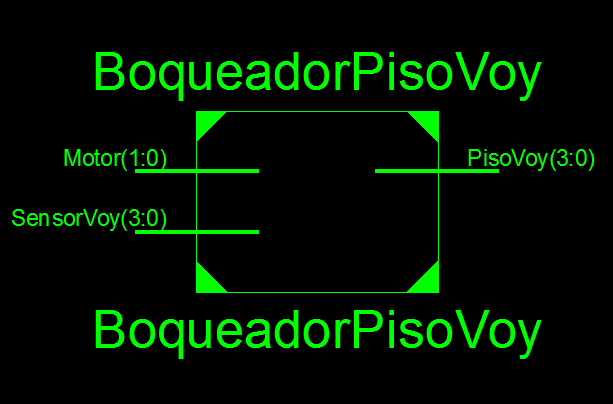
\includegraphics[width = 0.6\textwidth ]{BloqueBloqueadorPisoVoyOK}
		    \caption{Esquema exterior del bloque Bloqueador PisoVoy}
		    \label{fig:BloqueBloqueadorPisoVoyOK}
	\end{figure}
    Además podemos ver en la Figura (\ref{fig:BloqueBloqueadorPisoVoyImplementacion}) como se compone internamente el bloque, como se codifica en hardware esta utilidad:
    \begin{figure}[H]
		    \centering
		    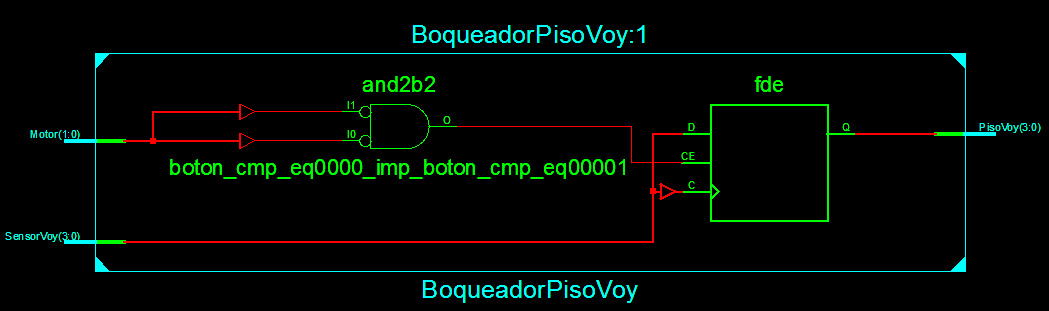
\includegraphics[width = 0.9\textwidth ]{BloqueBloqueadorPisoVoyImplementacion}
		    \caption{Esquema interno del bloque Bloqueador PisoVoy}
		    \label{fig:BloqueBloqueadorPisoVoyImplementacion}
	\end{figure}

\subsection{Código Bloque \textit{Bloqueador PisoVoy (testbench)}:} \label{code:BloqueadorpisoVoy_tb}
    \inputminted[frame=lines,fontsize=\footnotesize,linenos]{vhdl}{CodeFiles/BloqueadorPisoVoy_tb.vhd}

    Utilizando este testbench se obtiene el comportamiento que se puede ver en la Figura (\ref{fig:SimulacionBloqueadorPisoVoy}):

    \begin{figure}[H]
		    \centering
		    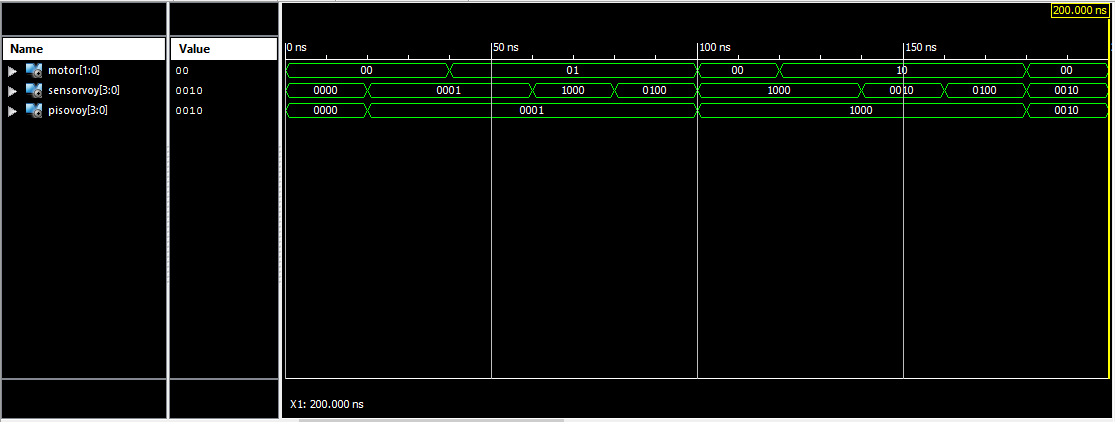
\includegraphics[width = 0.8\textwidth ]{SimulacionBloqueadorPisoVoy}
		    \caption{Simulación del testbench del bloque BloqueadorPisoVoy}
		    \label{fig:SimulacionBloqueadorPisoVoy}
	\end{figure}

\subsection{Código Bloque \textit{Decodificador Binario a Entero}:} \label{code:DecodificadorBinarioEntero}
	Como se ha visto en la sección (\ref{bloque:DecodificadorBinarioEntero}) este bloque pasa de la codificación binaria que se ha dado a cada piso a su equivalente entero para su posterior comparación. Se puede ver el código de dicho bloque a continuación: \\ 

    \inputminted[frame=lines,fontsize=\footnotesize,linenos]{vhdl}{CodeFiles/DecodificadorBinarioEntero.vhd}
    
    Como se puede ver en la Figura (\ref{fig:BloqueDecodificadorBinarioEnteroOK}) el esquema obtenido una vez programado y sintetizado se corresponde con el que se pretendía.
    \begin{figure}[H]
		    \centering
		    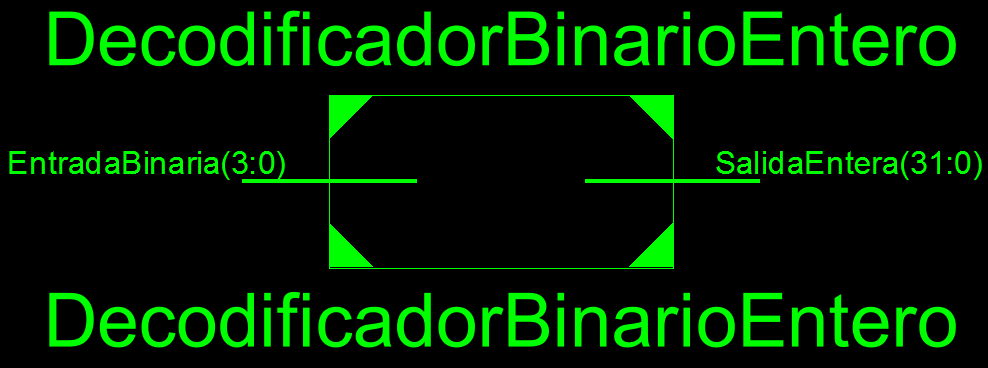
\includegraphics[width = 0.6\textwidth ]{BloqueDecodificadorBinarioEnteroOK}
		    \caption{Esquema exterior del bloque Decodificador Binario-Entero}
		    \label{fig:BloqueDecodificadorBinarioEnteroOK}
	\end{figure}
    Además podemos ver en la Figura (\ref{fig:BloqueDecodificadorBinarioEnteroImplementacion}) como se compone internamente el bloque, como se codifica en hardware esta utilidad:
    \begin{figure}[H]
		    \centering
		    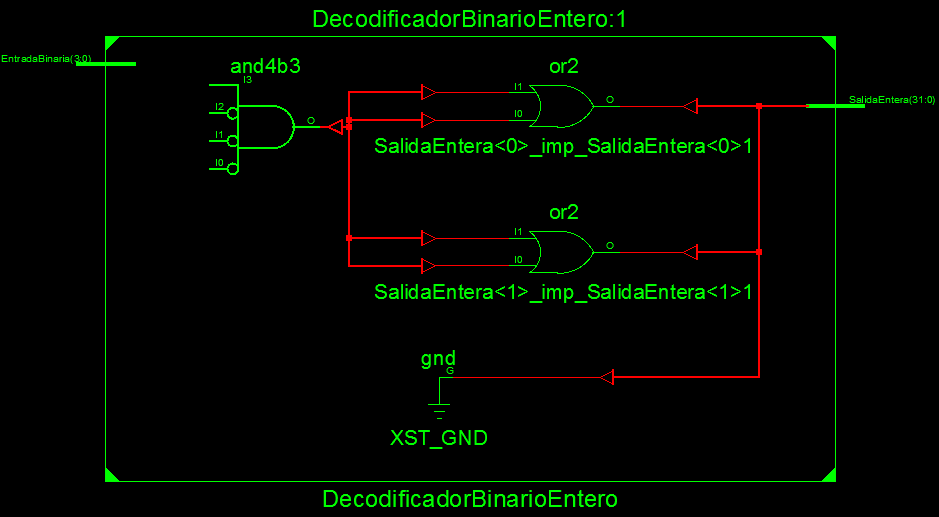
\includegraphics[width = 0.9\textwidth ]{BloqueDecodificadorBinarioEnteroImplementacion}
		    \caption{Esquema interno del bloque Decodificador Binario-Entero}
		    \label{fig:BloqueDecodificadorBinarioEnteroImplementacion}
	\end{figure}
    
\subsection{Código Bloque \textit{Decodificador Binario a Entero (testbench)}:} \label{code:DecodificadorBinarioEntero_tb}
    \inputminted[frame=lines,fontsize=\footnotesize,linenos]{vhdl}{CodeFiles/DecodificadorBinarioEntero_tb.vhd}

    Utilizando este testbench se obtiene el comportamiento que se puede ver en la Figura (\ref{fig:SimulacionDecodificadorBinarioEntero}):

    \begin{figure}[H]
		    \centering
		    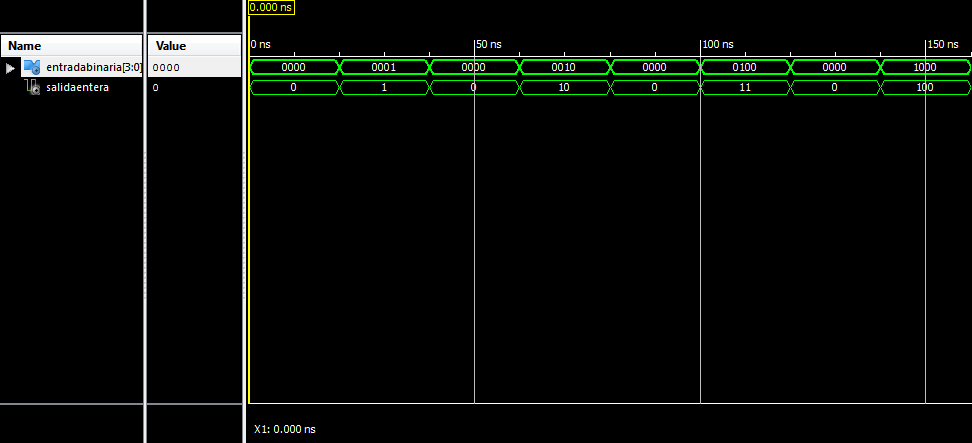
\includegraphics[width = 0.8\textwidth ]{SimulacionDecodificadorBinarioEntero}
		    \caption{Simulación del testbench del bloque DecodificadorBinarioEntero}
		    \label{fig:SimulacionDecodificadorBinarioEntero}
	\end{figure}

\subsection{Código Bloque \textit{Comparador}:} \label{code:Comparador}
	Como se ha visto en la seccion (\ref{bloque:Comparado}) este bloque compara las dos señales enteras; si el piso objetivo está por encima del actual el motor sube y la puerta se cierra, si el piso objetivo es igual al piso actual el motor está parado y la puerta abierta, y finalmente, si el piso objetivo es menor que el piso actual el motor baja manteniendo la puerta cerrada durante el proceso. A continuación se presenta el código del bloque: \\ 

    \inputminted[frame=lines,fontsize=\footnotesize,linenos]{vhdl}{CodeFiles/Comparador.vhd}	

	Como se puede ver en la Figura (\ref{fig:BloqueComparadorOK}) el esquema obtenido una vez programado y sintetizado se corresponde con el que se pretendía.
    \begin{figure}[H]
		    \centering
		    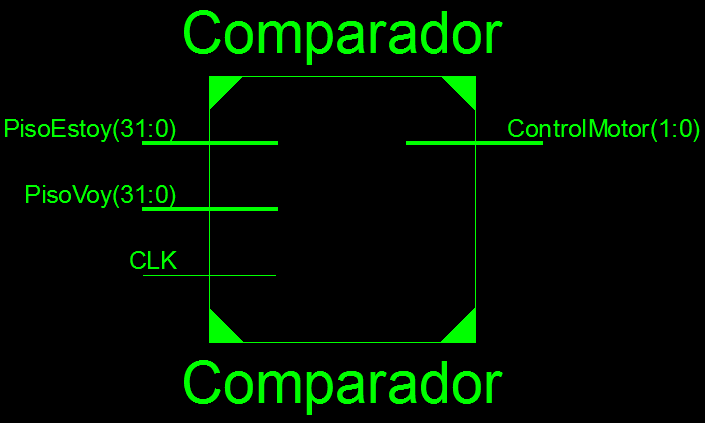
\includegraphics[width = 0.6\textwidth ]{BloqueComparadorOK}
		    \caption{Esquema exterior del Bloque Comparador}
		    \label{fig:BloqueComparadorOK}
	\end{figure}
    Además podemos ver en la Figura (\ref{fig:BloqueComparadorImplementacion}) como se compone internamente el bloque, como se codifica en hardware esta utilidad:
    \begin{figure}[H]
		    \centering
		    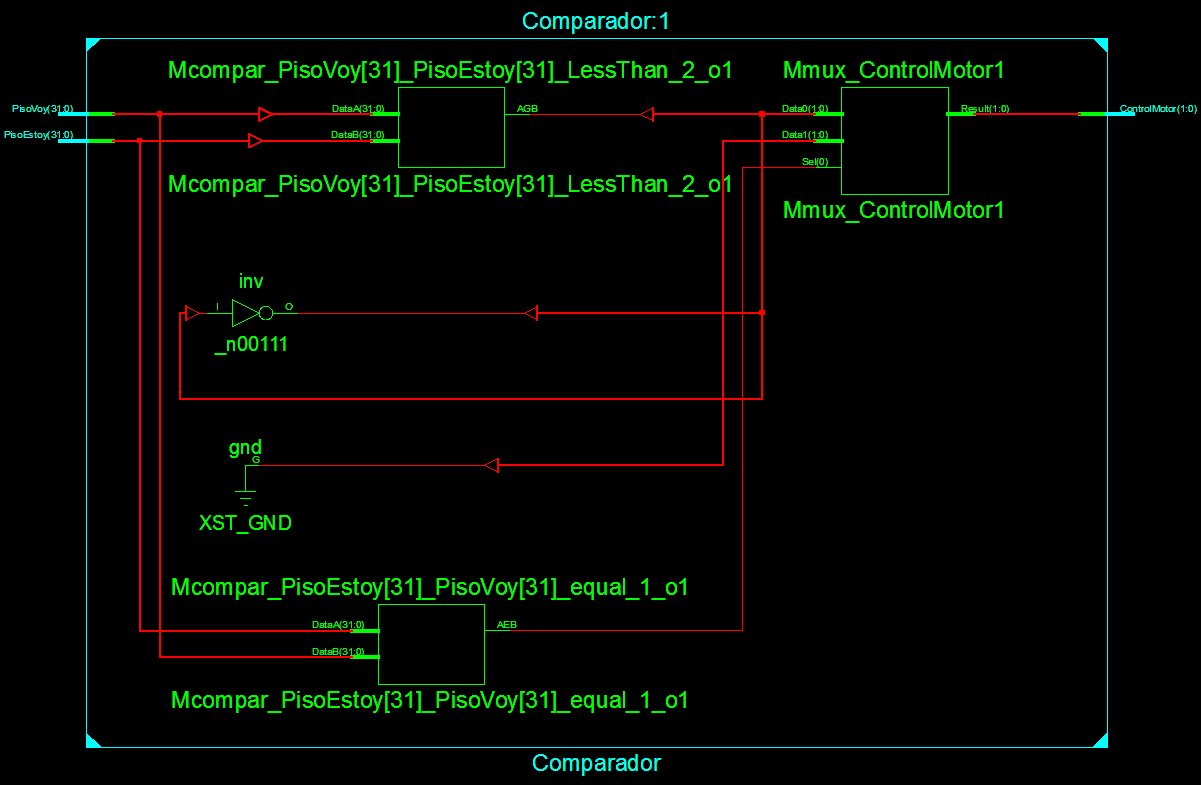
\includegraphics[width = 0.9\textwidth ]{BloqueComparadorImplementacion}
		    \caption{Esquema interno del Bloque Comparador}
		    \label{fig:BloqueComparadorImplementacion}
	\end{figure}

\subsection{Código Bloque \textit{Comparador (testbench)}:} \label{code:Comparador_tb}
    \inputminted[frame=lines,fontsize=\footnotesize,linenos]{vhdl}{CodeFiles/Comparador_tb.vhd}

    Utilizando este testbench se obtiene el comportamiento que se puede ver en la Figura (\ref{fig:SimulacionComparador}):

    \begin{figure}[H]
		    \centering
		    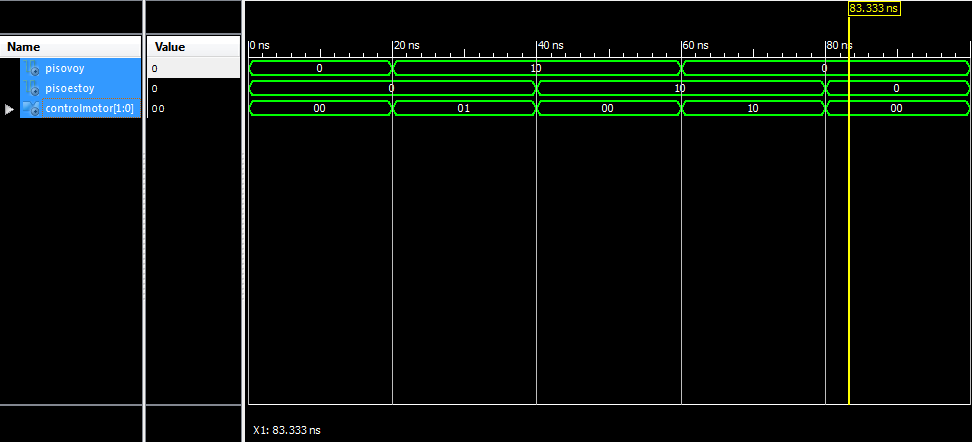
\includegraphics[width = 0.8\textwidth ]{SimulacionComparador}
		    \caption{Simulación del testbench del bloque Comparador}
		    \label{fig:SimulacionComparador}
	\end{figure}

\subsection{Código Bloque \textit{ Simulacion Motor Puerta}:} \label{code:MotorPuerta}
	Como se ha visto en la sección (\ref{boque:MotorPuerta}) al no tener motor y puerta reales se ha optado por sacar su reacción a traves de los displays. Este bloque es similar al bloque Decodificador7s (se puede encontrar la descripción en la seccion \ref{bloque:Decodificador7s} así como su codificación en la sección \ref{code:Decodificador7s} para observar las similitudes). Lo que hace es tomar la señal de entrada de dos bits, que codifica la reacción del motor y la puerta para transformarla en un caracter que se podrá mostrar a través del display de 7 segmentos. La codificación en VHDL se puede ver a continuación: \\ 

	\inputminted[frame=lines,fontsize=\footnotesize,linenos]{vhdl}{CodeFiles/MotorPuerta.vhd}

	Como se puede ver en la Figura (\ref{fig:MotorPuertaOK}) el esquema obtenido una vez programado y sintetizado se corresponde con el que se pretendía.
    \begin{figure}[H]
		    \centering
		    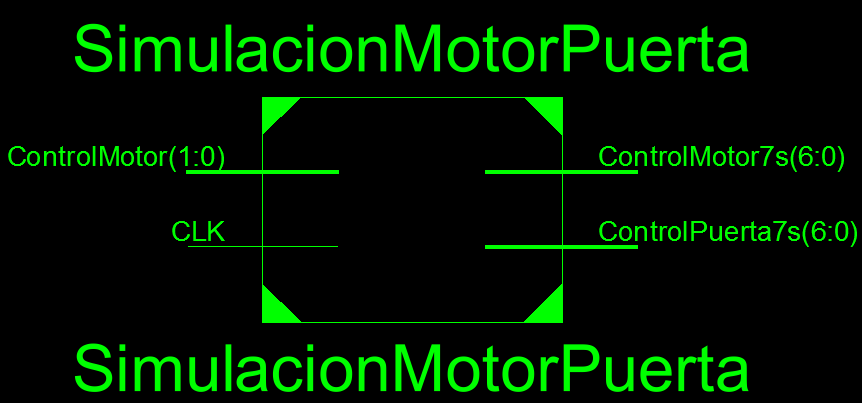
\includegraphics[width = 0.6\textwidth ]{MotorPuertaOK}
		    \caption{Esquema exterior del simulador Motor Puerta}
		    \label{fig:MotorPuertaOK}
	\end{figure}
    Además podemos ver en la Figura (\ref{fig:MotorPuertaImplementacion}) como se compone internamente el bloque, como se codifica en hardware esta utilidad:
    \begin{figure}[H]
		    \centering
		    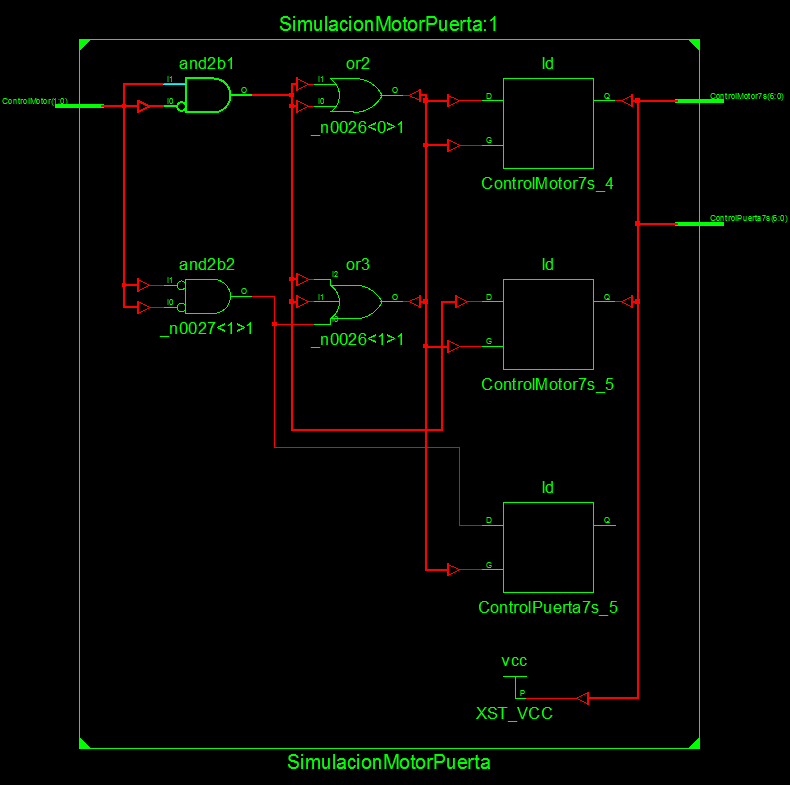
\includegraphics[width = 0.9\textwidth ]{MotorPuertaImplementacion}
		    \caption{Esquema interno del simulador Motor Puerta}
		    \label{fig:MotorPuertaImplementacion}
	\end{figure}
\subsection{Código Bloque \textit{Simulacion Motor Puerta (testbench)}:} \label{code:MotorPuerta_tb}
	\inputminted[frame=lines,fontsize=\footnotesize,linenos]{vhdl}{CodeFiles/MotorPuerta_tb.vhd}

    Utilizando este testbench se obtiene el comportamiento que se puede ver en la Figura (\ref{fig:SimulacionMotorPuerta}):

    \begin{figure}[H]
		    \centering
		    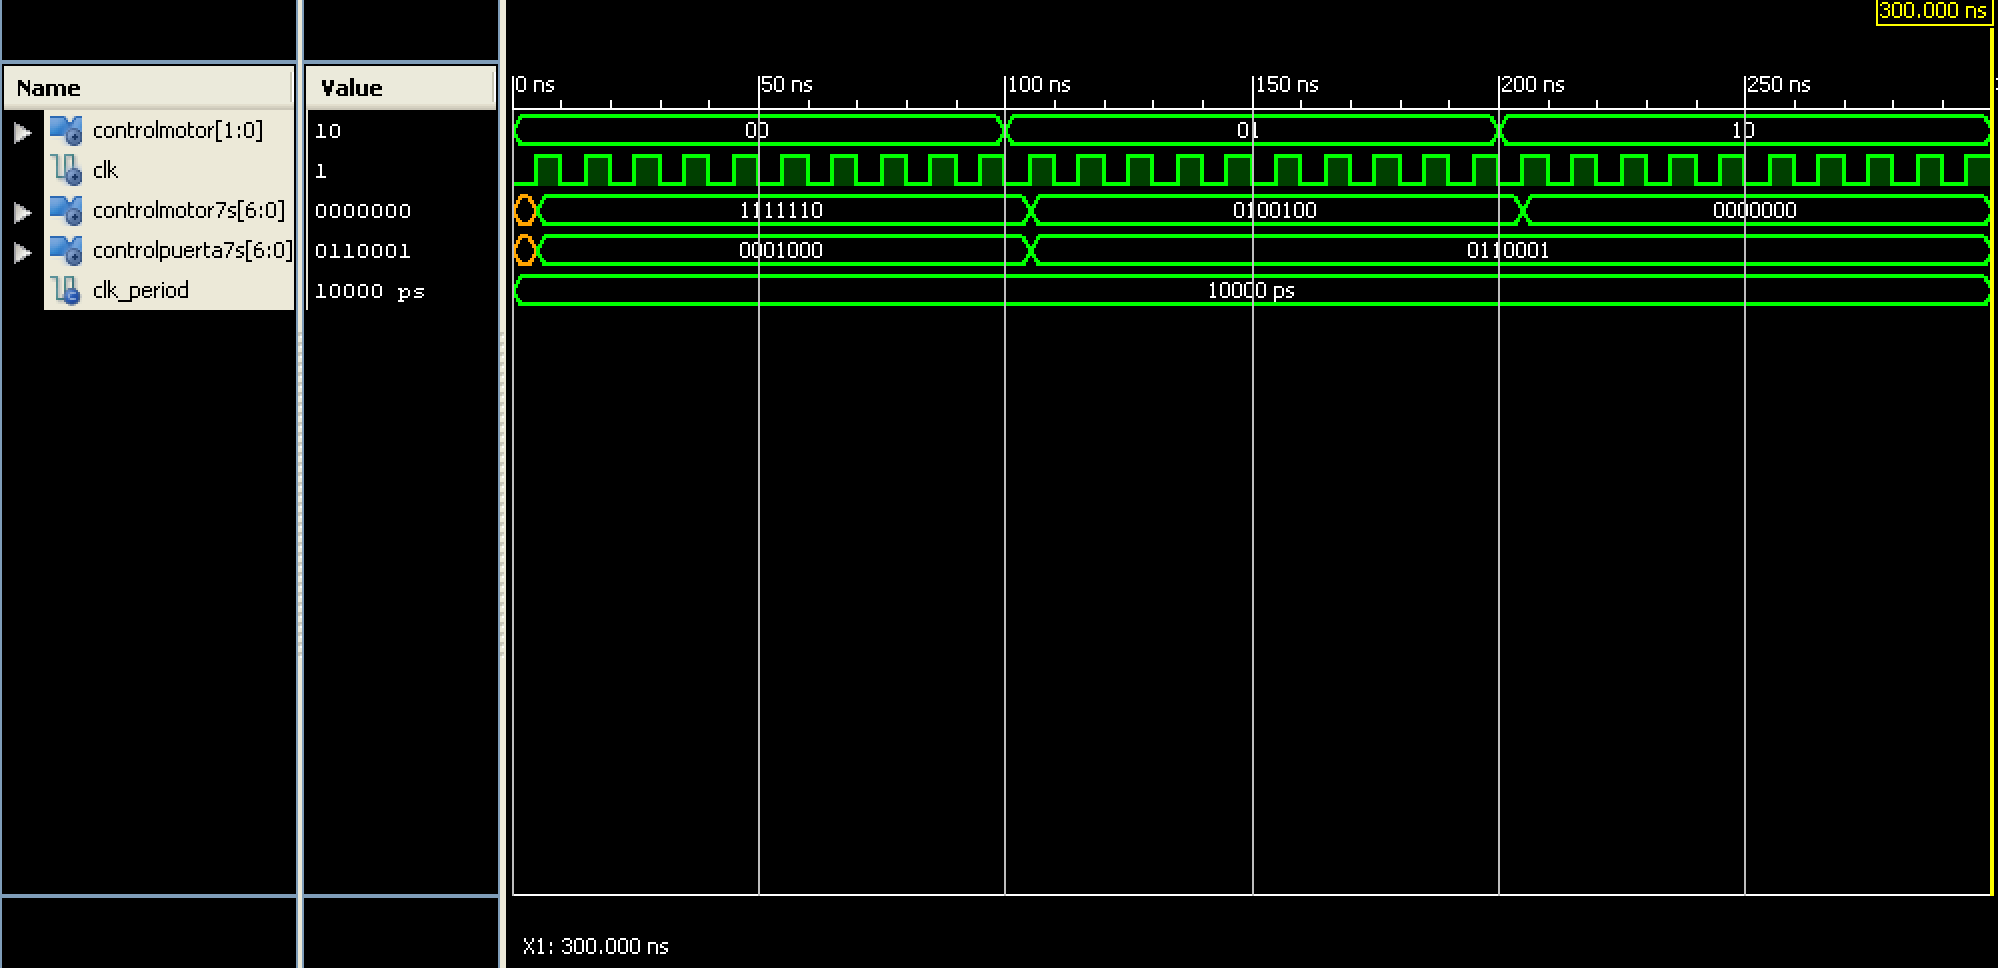
\includegraphics[width = 0.8\textwidth ]{SimulacionPuertaMotor}
		    \caption{Simulación del testbench del simulador MotorPuerta}
		    \label{fig:SimulacionMotorPuerta}
	\end{figure}

\subsection{Entidad \textit{Interfaz Entrada}:} \label{code:InterfazEntrada}
	\inputminted[frame=lines,fontsize=\footnotesize,linenos]{vhdl}{CodeFiles/EntidadInterfazEntrada.vhd}

	Como se puede ver en la Figura (\ref{fig:EntidadInterfazEntradaOK}) el esquema obtenido una vez programado y sintetizado se corresponde con el que se pretendía.
    \begin{figure}[H]
		    \centering
		    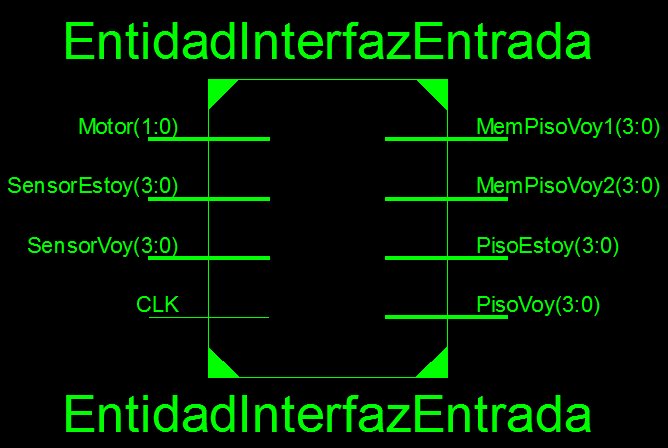
\includegraphics[width = 0.6\textwidth ]{EntidadInterfazEntradaOK}
		    \caption{Esquema exterior de la Entidad InterfazEntrada}
		    \label{fig:EntidadInterfazEntradaOK}
	\end{figure}
    Además podemos ver en la Figura (\ref{fig:EntidadInterfazEntradaImplementacion}) como se compone internamente el bloque, como se codifica en hardware esta utilidad:
    \begin{figure}[H]
		    \centering
		    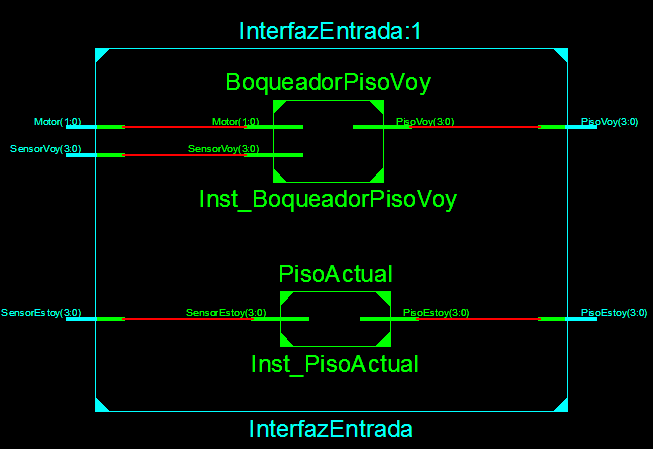
\includegraphics[width = 0.9\textwidth ]{EntidadInterfazEntradaImplementacion}
		    \caption{Esquema interno de la Entidad InterfazEntrada}
		    \label{fig:EntidadInterfazEntradaImplementacion}
	\end{figure}

\subsection{Código Entidad \textit{Interfaz Entrada (testbench)}:} \label{code:InterfazEntrada_tb}
	\inputminted[frame=lines,fontsize=\footnotesize,linenos]{vhdl}{CodeFiles/EntidadInterfazEntrada_tb.vhd}

    Utilizando este testbench se obtiene el comportamiento que se puede ver en la Figura (\ref{fig:SimulacionEntidadInterfazEntrada}):

    \begin{figure}[H]
		    \centering
		    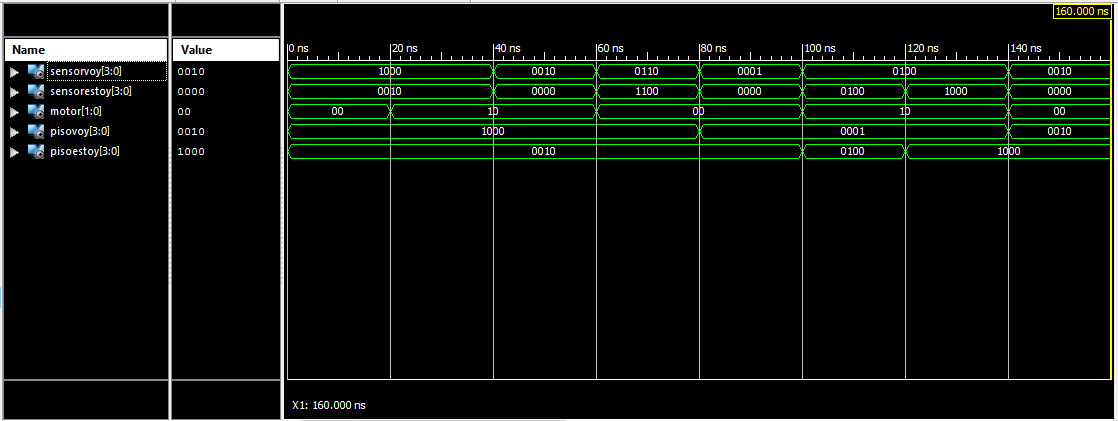
\includegraphics[width = 0.8\textwidth ]{SimulacionEntidadInterfazEntrada}
		    \caption{Simulación del testbench de la entidad InterfazEntrada}
		    \label{fig:SimulacionEntidadInterfazEntrada}
	\end{figure}

\subsection{Código Entidad \textit{Control Ascensor}:} \label{code:ControlAscensor}
	Como se ha explicado en la sección (\ref{bloque:ControlAscensor}) esta entidad coordina y encapsula lo necesario para la toma de decisiones llevada a cabo por nuestro sistema, esto incluye el comparador y el codificador de binario a entero vistos anteriormente. \\ 

	\inputminted[frame=lines,fontsize=\footnotesize,linenos]{vhdl}{CodeFiles/EntidadControlAscensor.vhd}

	Como se puede ver en la Figura (\ref{fig:EntidadControlAscensorOK}) el esquema obtenido una vez programado y sintetizado se corresponde con el que se pretendía.
    \begin{figure}[H]
		    \centering
		    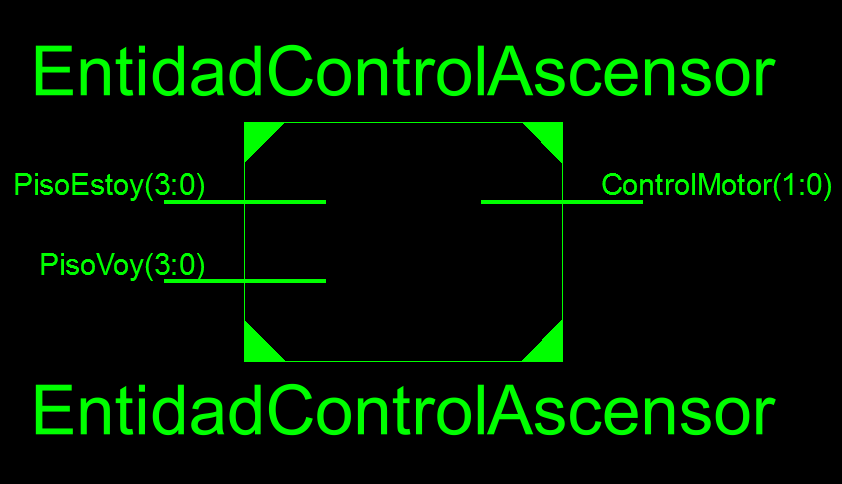
\includegraphics[width = 0.6\textwidth ]{EntidadControlAscensorOK}
		    \caption{Esquema exterior de la Entidad ControlAscensor}
		    \label{fig:EntidadControlAscensorOK}
	\end{figure}
    Además podemos ver en la Figura (\ref{fig:EntidadControlAscensorImplementacion}) como se compone internamente el bloque, como se codifica en hardware esta utilidad:
    \begin{figure}[H]
		    \centering
		    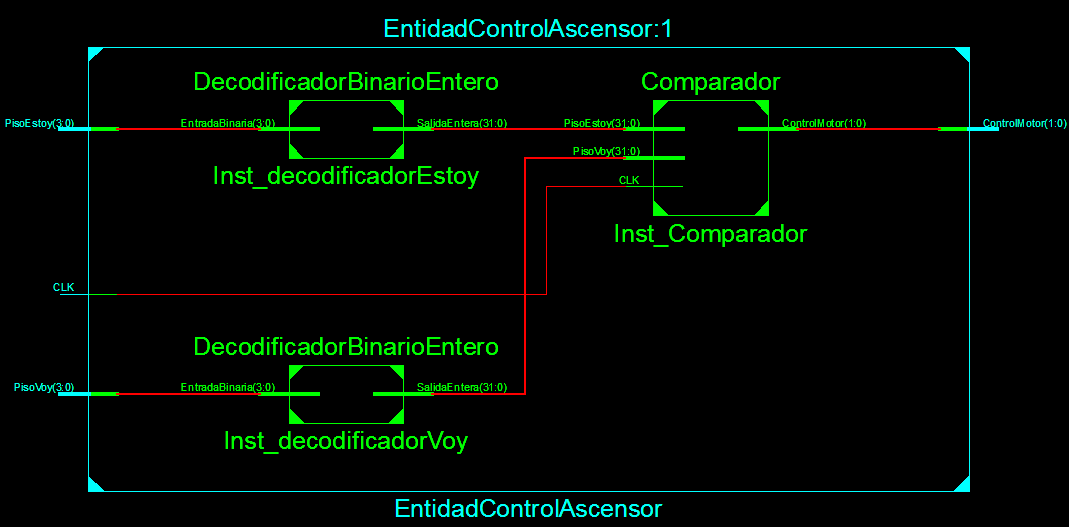
\includegraphics[width = 0.9\textwidth ]{EntidadControlAscensorImplementacion}
		    \caption{Esquema interno de la Entidad ControlAscensor}
		    \label{fig:EntidadControlAscensorImplementacion}
	\end{figure}

\subsection{Código Entidad \textit{Control Ascensor (testbench)}:} \label{code:ControlAscensor_tb}
	\inputminted[frame=lines,fontsize=\footnotesize,linenos]{vhdl}{CodeFiles/EntidadControlAscensor_tb.vhd}

    Utilizando este testbench se obtiene el comportamiento que se puede ver en la Figura (\ref{fig:SimulacionEntidadControlAscensor}):

    \begin{figure}[H]
		    \centering
		    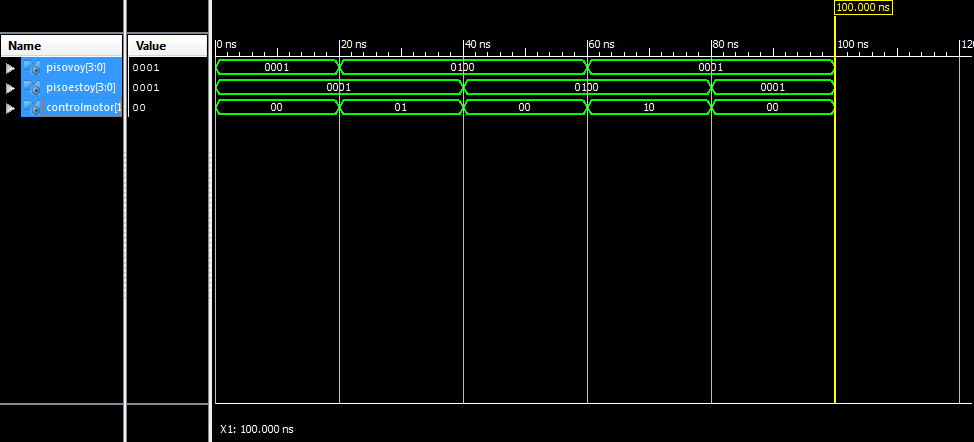
\includegraphics[width = 0.8\textwidth ]{SimulacionEntidadControlAscensor}
		    \caption{Simulación del testbench de la entidad ControlAscensor}
		    \label{fig:SimulacionEntidadControlAscensor}
	\end{figure}

\subsection{Código Entidad \textit{Visualizacion}:} \label{code:Visualizacion}

Esta entidad, formada por tres bloques, dos Decodificador7s y un DivisorFrecuencia se encarga de mostrar en las cuatro pantallas de siete segmentos el estado del ascensor. \\ 
	\inputminted[frame=lines,fontsize=\footnotesize,linenos]{vhdl}{CodeFiles/EntidadVisualizacion.vhd}

	Como se puede ver en la Figura (\ref{fig:EntidadControlAscensorOK}) el esquema obtenido una vez programado y sintetizado se corresponde con el que se pretendía.
    \begin{figure}[H]
		    \centering
		    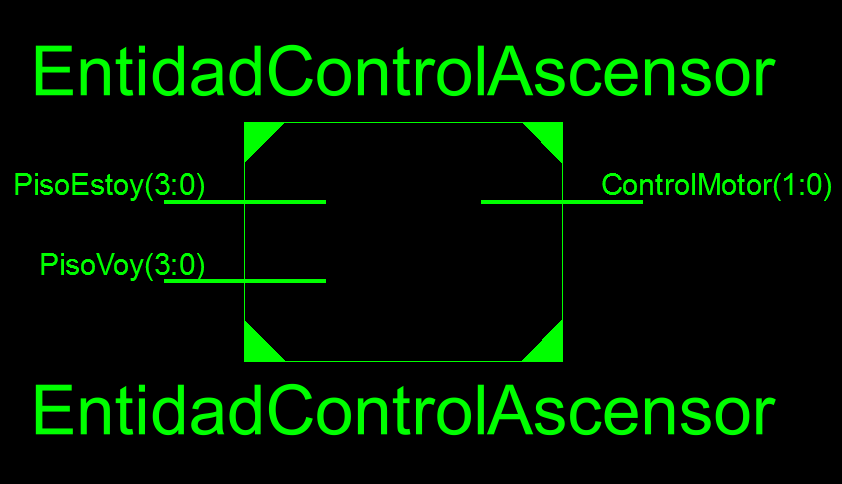
\includegraphics[width = 0.6\textwidth ]{EntidadControlAscensorOK}
		    \caption{Esquema exterior de la Entidad Visualizacion}
		    \label{fig:EntidadVisualizacionOK}
	\end{figure}
    Además podemos ver en la Figura (\ref{fig:EntidadVisualizacionImplementacion}) como se compone internamente el bloque, como se codifica en hardware esta utilidad:
    \begin{figure}[H]
		    \centering
		    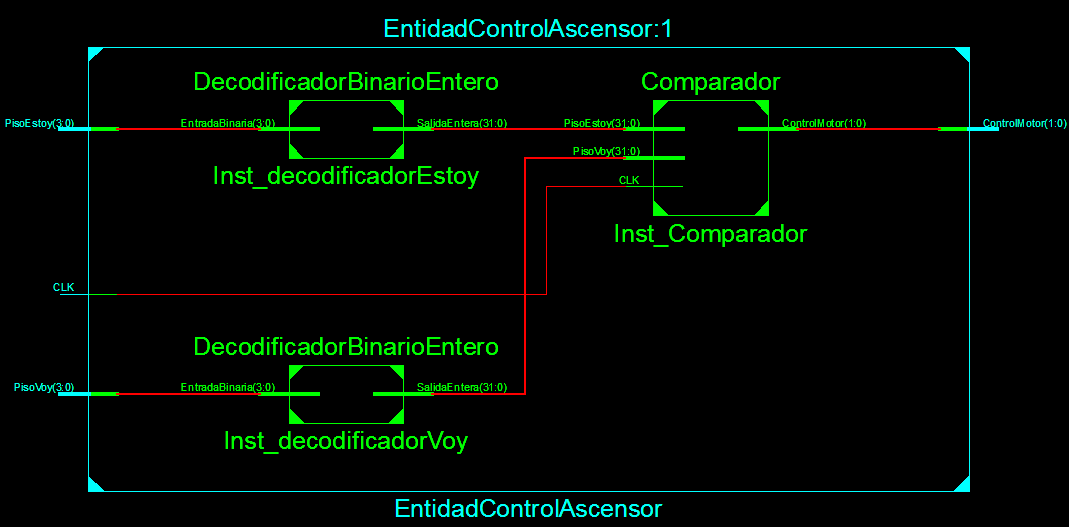
\includegraphics[width = 0.9\textwidth ]{EntidadControlAscensorImplementacion}
		    \caption{Esquema interno de la Entidad ControlAscensor}
		    \label{fig:EntidadVisualizacionImplementacion}
	\end{figure}

\subsection{Código Entidad \textit{Visualizacion (testbench)}:} \label{code:Visualizacion_tb}
	\inputminted[frame=lines,fontsize=\footnotesize,linenos]{vhdl}{CodeFiles/EntidadControlAscensor_tb.vhd}

    Utilizando este testbench se obtiene el comportamiento que se puede ver en la Figura (\ref{fig:SimulacionEntidadVisualizacion}):

    \begin{figure}[H]
		    \centering
		    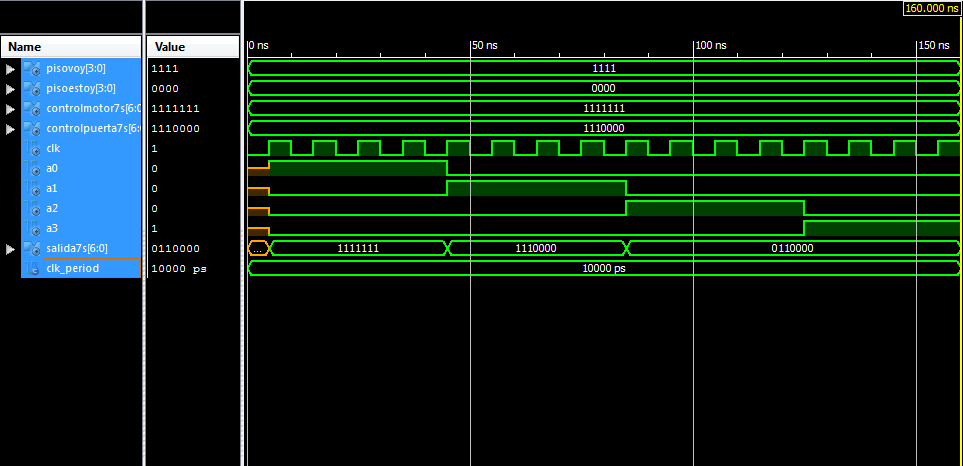
\includegraphics[width = 0.8\textwidth ]{SimulacionEntidadVisualizacion}
		    \caption{Simulación del testbench de la entidad ControlAscensor}
		    \label{fig:SimulacionEntidadVisualizacion}
	\end{figure}


\subsection{Código Código Entidad \textit{Acensor}:} \label{code:Acensor}

\subsection{Código Código Entidad \textit{Acensor (testbench)}:} \label{code:Acensor_tb}
 %importa el fichero Codigo.tex
    
    \section{Pruebas en placa y análisis de resultados:} \label{section:PruebasYResultados}

    		\begin{table}[H]
    \centering
		\begin{tabular}{|c|c|c||c|c|c|}
			\hline
			\rowcolor[rgb]{0.21,0.69,0.87}\multicolumn{6}{|c|}{  \textbf{ {Configuración Pines de entrada}}} \\
			\hline \hline
			\multicolumn{3}{|c|}{  \textbf{ {SensorVoy (4bits)}}} & \multicolumn{3}{|c|}{\textbf{SensorEstoy (4bits)}} \\
			\hline
			SensorVoy[0] & SW0 & F12 & SensorEstoy[0] & BTN0 & M13 \\
			\hline
			SensorVoy[1] & SW1 & G12 & SensorEstoy[1] & BTN1 & M14 \\
			\hline
			SensorVoy[2] & SW2 & H14 & SensorEstoy[2] & BTN2 & L13 \\
			\hline
			SensorVoy[3] & SW3 & H13 & SensorEstoy[3] & BTN3 & L14 \\
			\hline
		\end{tabular}
		\caption{ Configuración de los pines de entrada con las entradas del sistema }
		\label{tab:pinEntradas}
	\end{table}

	\begin{table}[H]
    \centering
		\begin{tabular}{|c|c|}
			\hline
			\rowcolor[rgb]{0.21,0.69,0.87}\multicolumn{2}{|c|}{  \textbf{ {Configuración pin CLK}}} \\
			\hline \hline
			CLK & T9 \\ 
			\hline
		\end{tabular}
		\caption{ Configuración del pin para el CLK }
		\label{tab:pinCLK}
	\end{table}

	\begin{table}[H]
    \centering
		\begin{tabular}{|c|c||c|c|c|}
			\hline
			\rowcolor[rgb]{0.21,0.69,0.87}\multicolumn{5}{|c|}{  \textbf{ {Configuración Pines de los displays de 7 segmentos}}} \\
			\hline \hline
			\multicolumn{2}{|c|}{  \textbf{ { Salida7s (7bits)}}} & \multicolumn{2}{|c|}{\textbf{Ánodos de Control}} \\
			\hline
			Salida7s[0] & P16 & Motor & AN0 & D14 \\
			\hline
			Salida7s[1] & N16 & Puerta & AN1 & G14 \\
			\hline
			Salida7s[2] & F13 & PisoVoy & AN2 & F14 \\
			\hline
			Salida7s[3] & R16 & PisoEstoy & AN3 & E13 \\
			\hline
			Salida7s[4] & P15 & - & - & - \\
			\hline
			Salida7s[5] & N15 & - & - & - \\
			\hline
			Salida7s[6] & G17 & - & - & - \\
			\hline
			Salida7s[7] & E14 & - & - & - \\
			\hline
		\end{tabular}
		\caption{ Configuración de los pines de salida al display de 7 segmentos }
		\label{tab:pin7s}
	\end{table}


	\begin{table}[H]
    \centering
		\begin{tabular}{|c|c|c|c|c|c|c|c|}
			\hline
			\rowcolor[rgb]{0.21,0.69,0.87}\multicolumn{8}{|c|}{  \textbf{ {Configuración Pines de los displays de 7 segmentos}}} \\
			\hline \hline
			LED[0] & LED[1] & LED[2] & LED[3] & LED[4] & LED[5] & LED[6] & LED[7] \\
			\hline			
			K12 & P14 & L12 & N14 & P13 & N12 & P12 & P11 \\
			\hline
		\end{tabular}
		\caption{ Configuración de los pines de los LEDs para las "memorias" }
		\label{tab:pinLEDs}
	\end{table}
	

\subsection{Caso de Uso Práctico:}
	
	Antes de poder hacer una comprobación del funcionamiento de la maqueta debemos conocer sobre que componentes se visualizará la información:
	
	\begin{figure}[H]
        \centering
        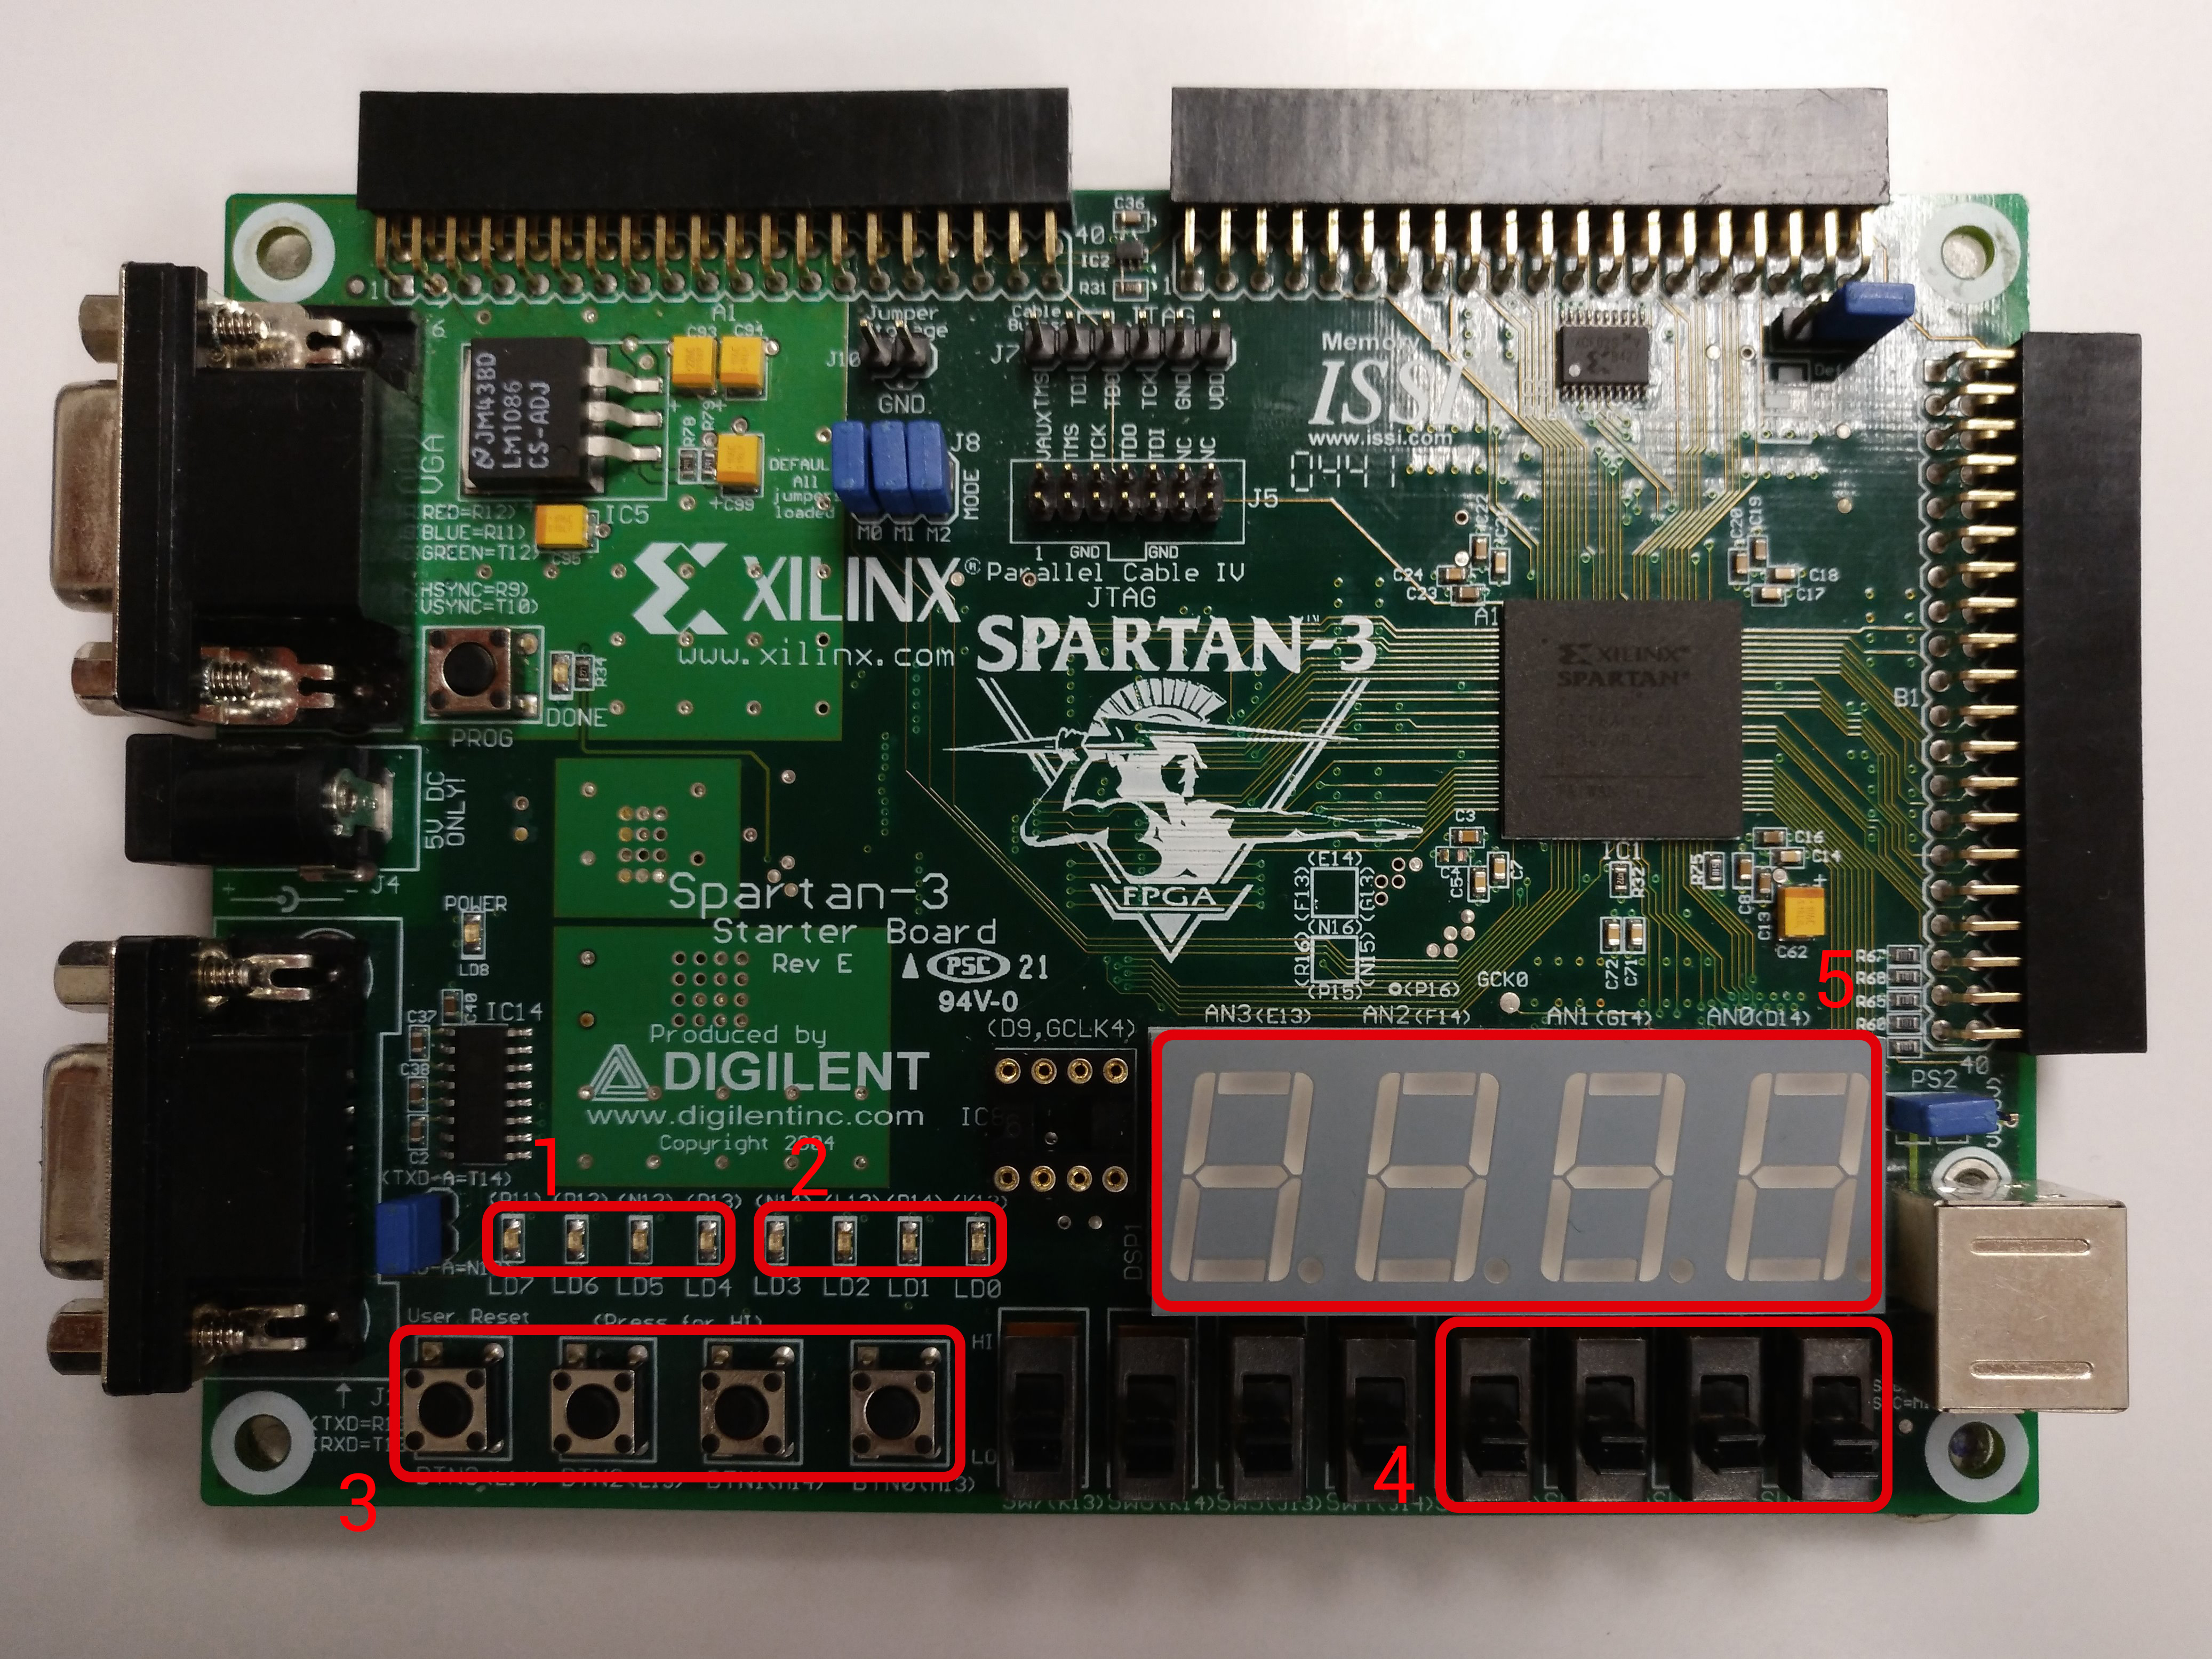
\includegraphics[width = 0.6\textwidth ]{CasoUso/0.jpg}
        \caption{Distribución salidas/entradas de la maqueta en la Spartan-3}
        \label{fig:Spartan3Interfaz}
    \end{figure}
    
    
    \begin{itemize}
	    \item 1. Memoria 2: se ve que piso se ha guardado iluminándose el LED de dicha posición (De derecha a izquierda en orden ascendente).
	    \item 2. Memoria 1: Equivalente al anterior, refleja la posición guardada en la memoria 1.
	    \item 3. Emulan los finales de carrera para ver en qué piso se encuentra el ascensor. De derecha a izquierda en orden ascendente de pisos.
	    \item 4. Emulan los botones para seleccionar el piso al que se desea ir. De derecha a izquierda en orden ascendente de pisos.
	    \item 5. Displays para mostrar la información, se puede ver a continuación que se muestra en cada display.
	\end{itemize} 
	
	\begin{figure}[H]
        \centering
        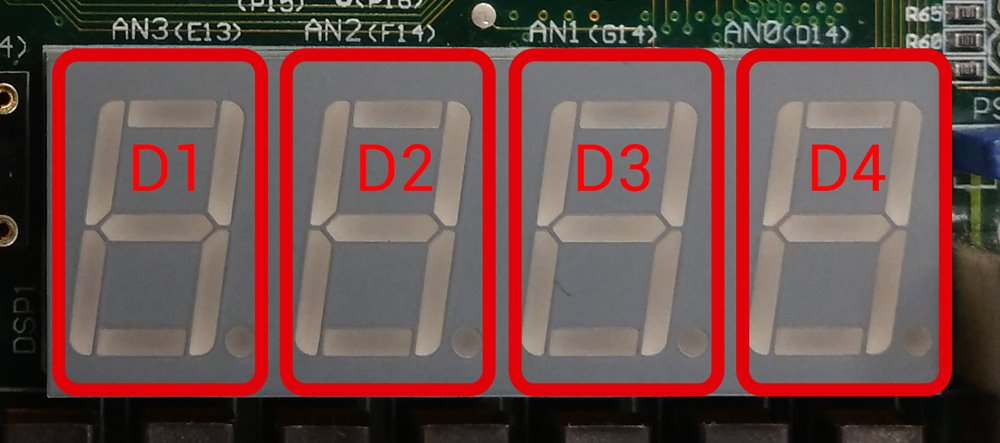
\includegraphics[width = 0.6\textwidth ]{CasoUso/0_1.jpg}
        \caption{Distibución de las salidas a los displays}
        \label{fig:Spartan3InterfazDisplays}
    \end{figure}
    
    \begin{itemize}
		    \item  D1. Piso actual, marcado por los finales de carrera.
		    \item  D2. Piso objetivo, al que quiero ir.
		    \item  D3. Funcionamiento de la puerta.
		    \item  D4. Funcionamiento del motor.
	\end{itemize} 
	
    
	\begin{table}[H]
	\centering
	\begin{tabular}{ccc}
		 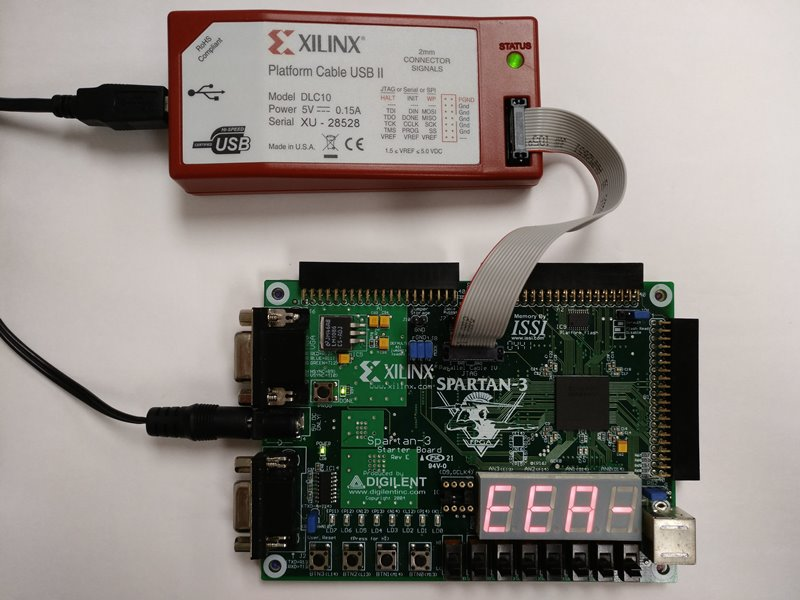
\includegraphics[width = 0.3\textwidth ]{CasoUso/2.jpg}  & 
		 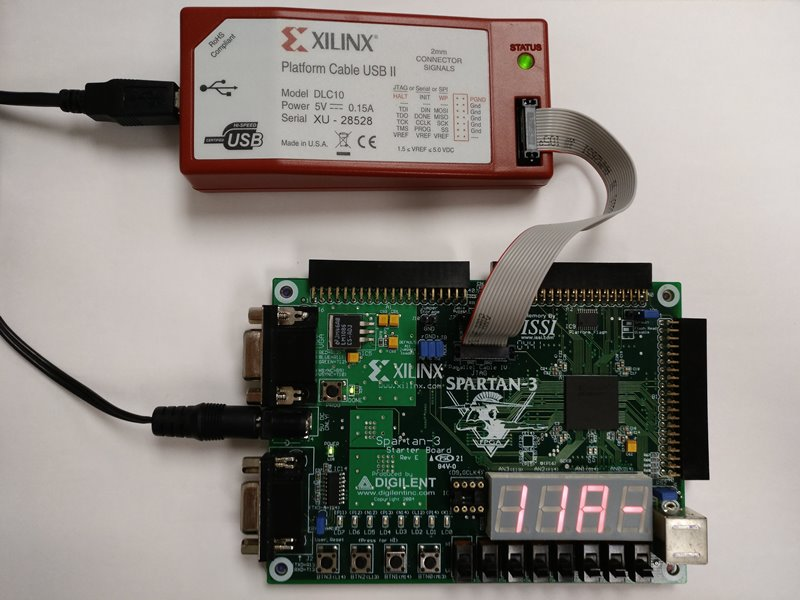
\includegraphics[width = 0.3\textwidth ]{CasoUso/3.jpg} & 
		 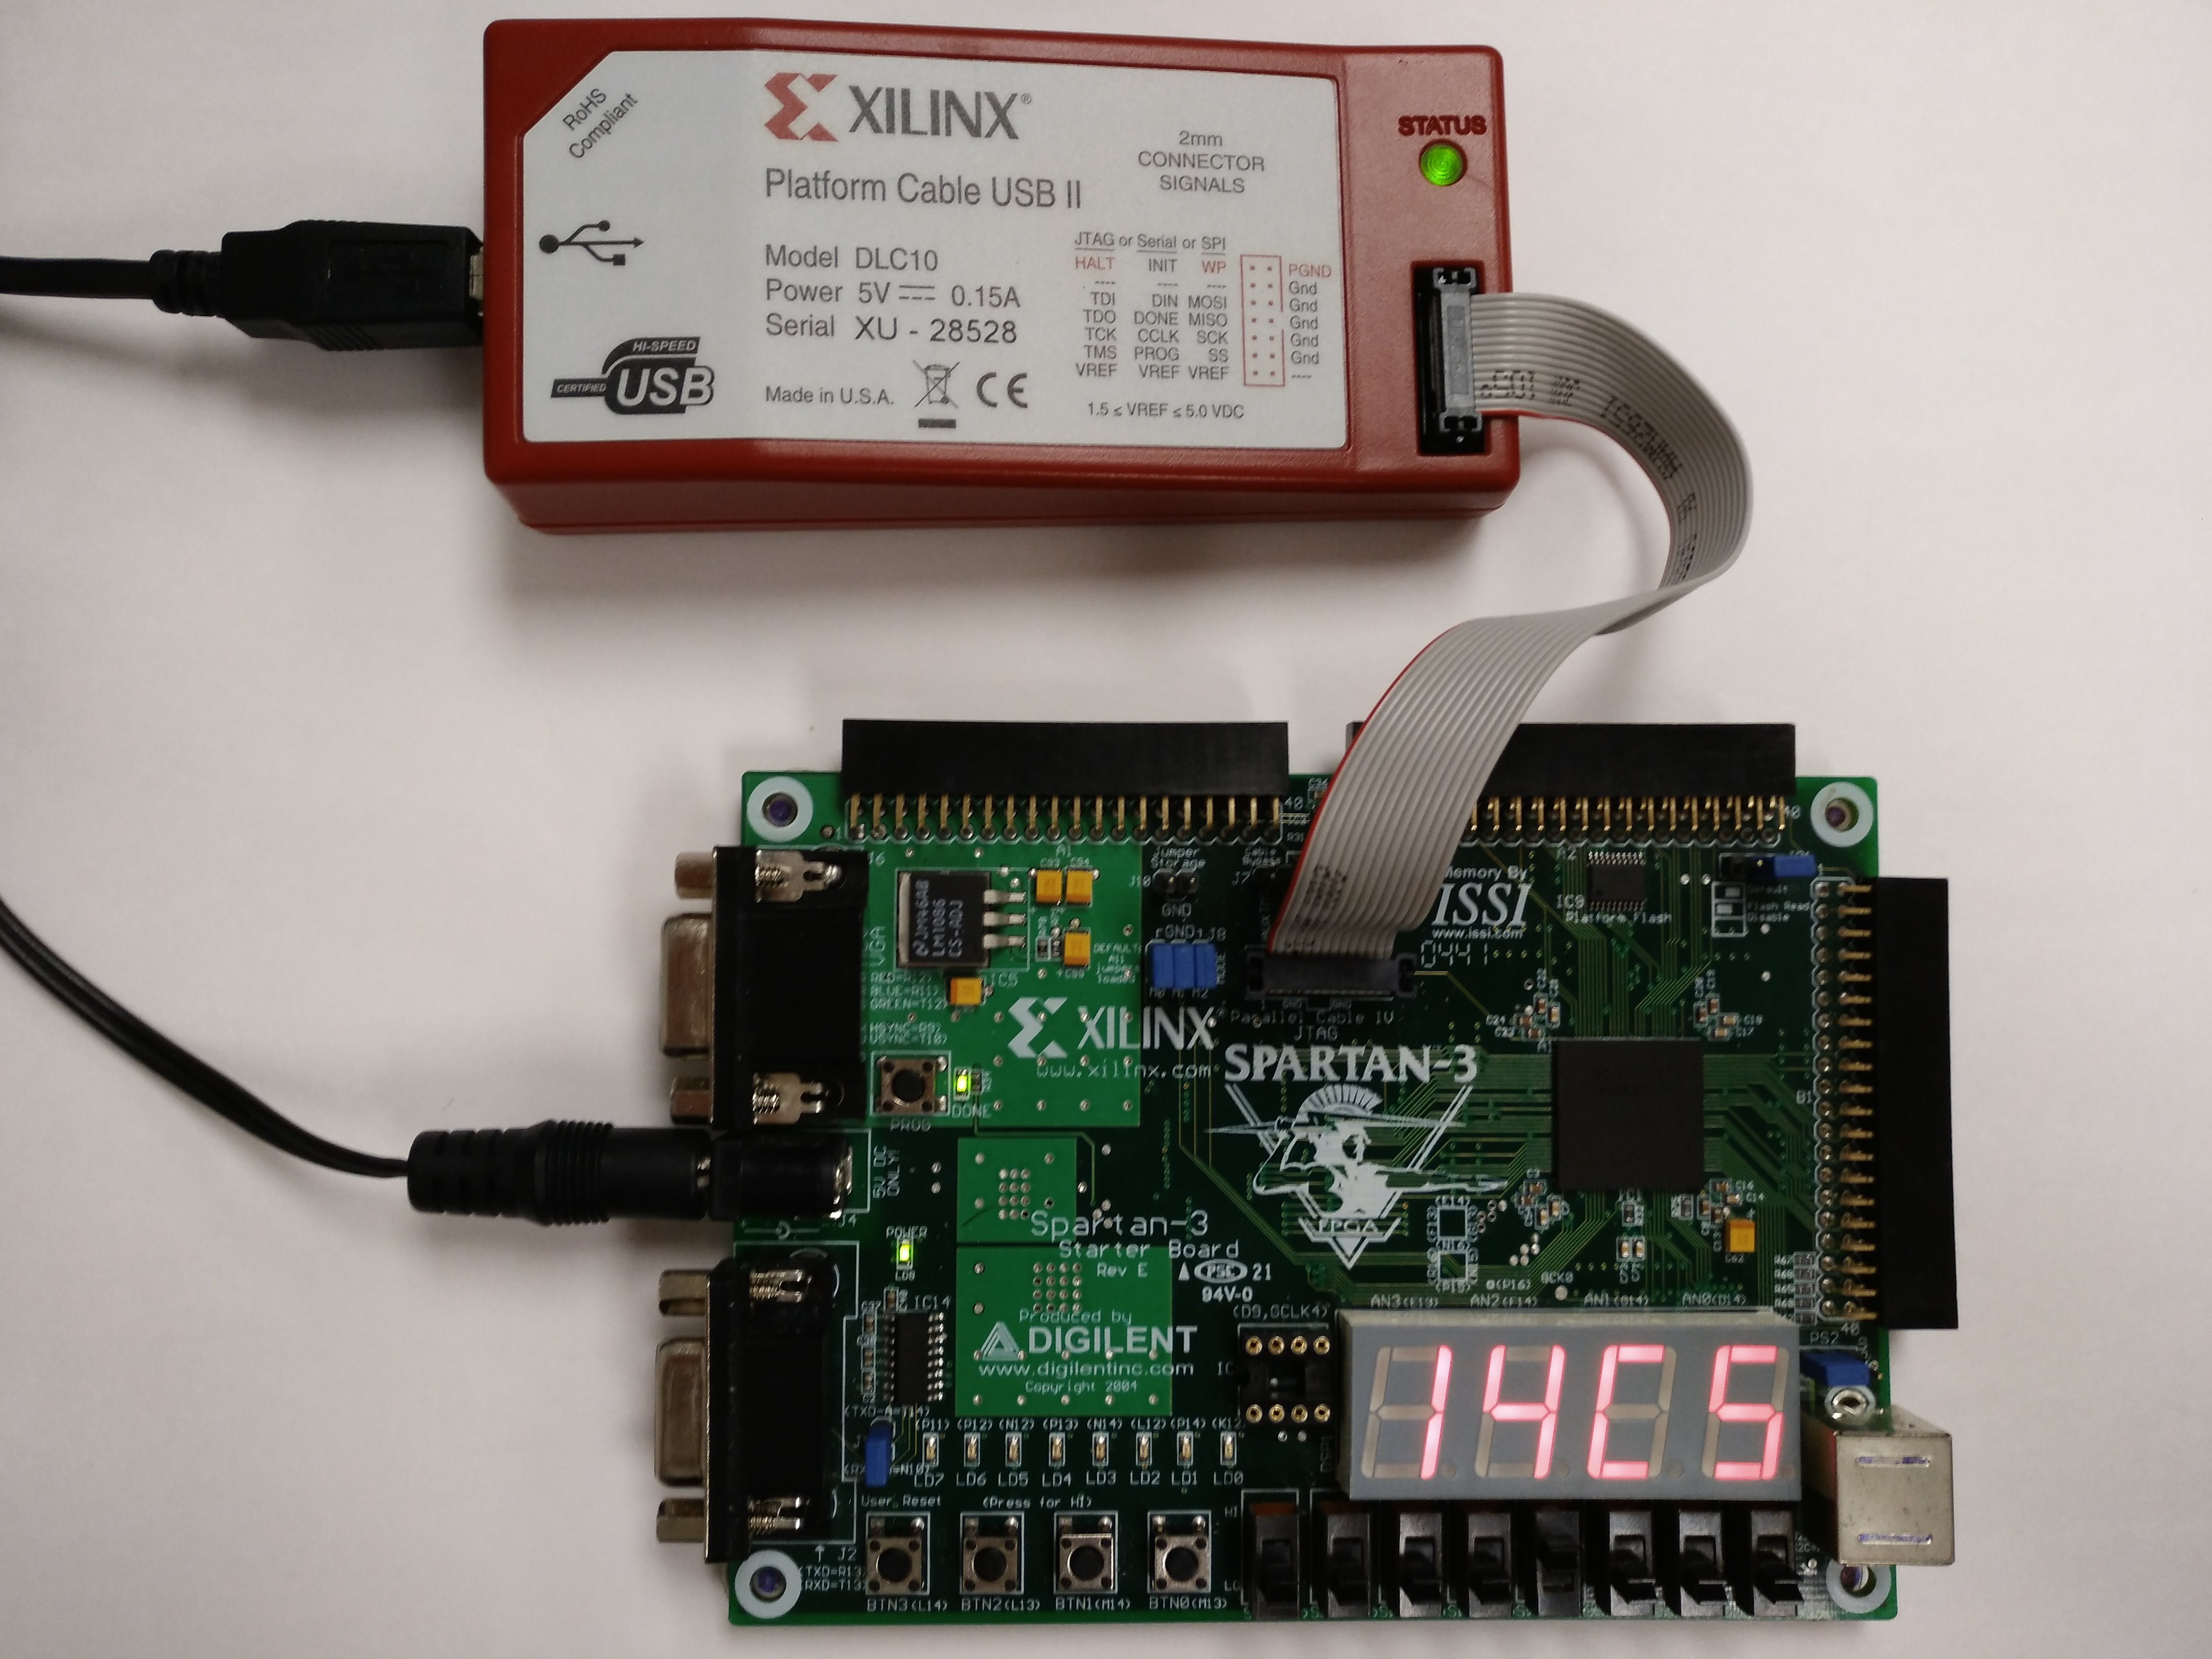
\includegraphics[width = 0.3\textwidth ]{CasoUso/4.jpg}   \\
	\end{tabular}
	\end{table}
	
	\begin{itemize}
	    \item 1. Al arrancar o resetear el sistema tanto el piso objetivo como el piso actual se inicializan a 0, a la espera de recibir información del sistema real. En este tipo de indeterminaciones el ascensor permanece parado con la puerta abierta.	
	    \item 2. Se pasa información sobre los pisos, en este caso el ascensor se situa en el primer piso. Tanto el piso actual como el objetivo son el mismo (1,1), el ascensor permanece parado (-) con la puerta abierta (A).	
	    \item 3. Se marca el cuarto piso como objetivo, la puerta se cierra (C) y el ascensor comienza a subir (S).
	\end{itemize}
	
	\begin{table}[H]
	\centering
	\begin{tabular}{ccc}
		  \includegraphics[width = 0.3\textwidth ]{CasoUso/5.jpg} &
		 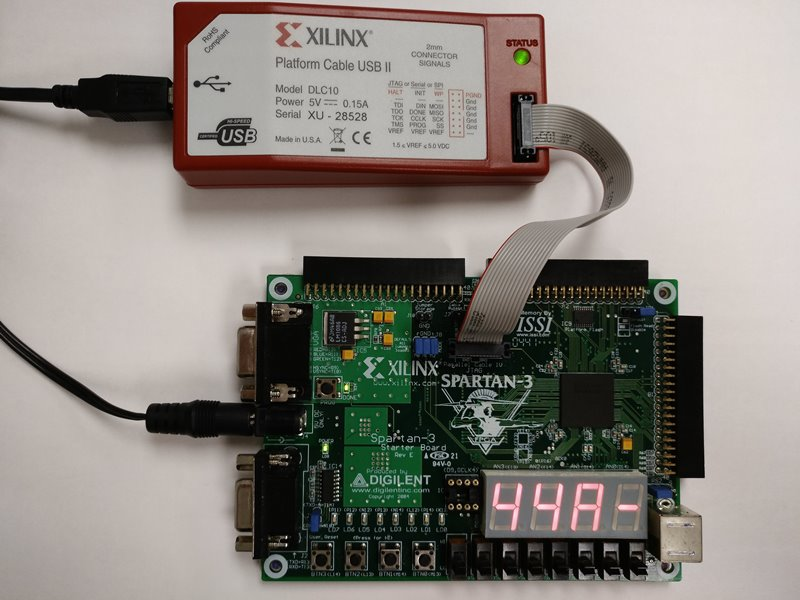
\includegraphics[width = 0.3\textwidth ]{CasoUso/6.jpg}  &
		  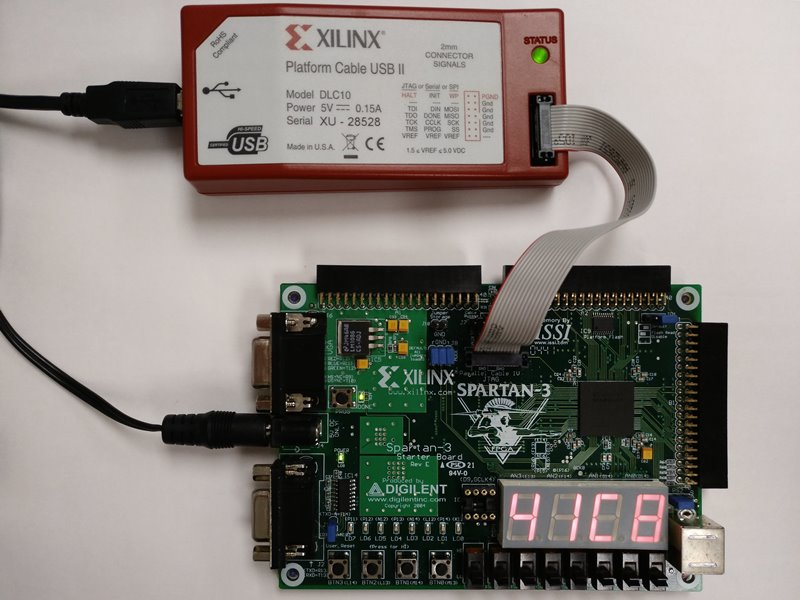
\includegraphics[width = 0.3\textwidth ]{CasoUso/7.jpg}   \\
	\end{tabular}
	\end{table}
	
	\begin{itemize}
	    \item 4. Según pasa por los pisos intermedios se actualiza el display de piso actual, el ascensor sigue cerrado y subiendo.	
	    \item 5.  Cuando llega a la planta deseada, el ascensor se detiene y la puerta se abre.	
	    \item 6.  Al marcar un piso inferior, el ascensor se cierra y comienza a descender (B).	
	\end{itemize}
	
	\begin{table}[H]
	\centering
	\begin{tabular}{ccc}
		 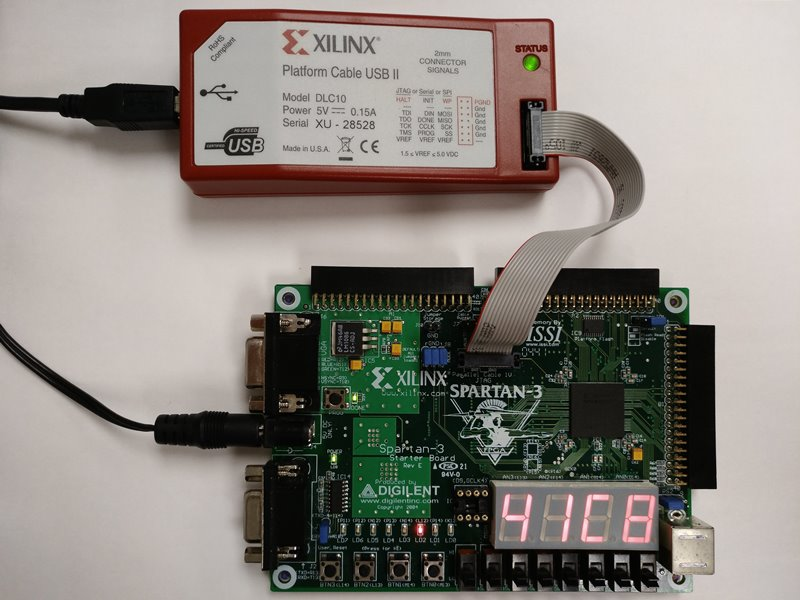
\includegraphics[width = 0.3\textwidth ]{CasoUso/8.jpg}   &
		 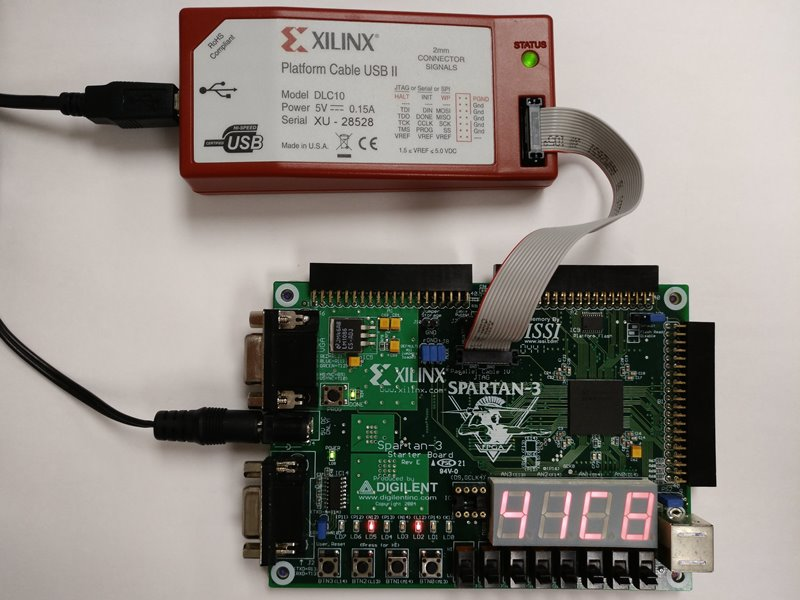
\includegraphics[width = 0.3\textwidth ]{CasoUso/9.jpg} &
		 \includegraphics[width = 0.3\textwidth ]{CasoUso/9_1.jpg}  \\
	\end{tabular}
	\end{table}
	
	\begin{itemize}
	    \item 7. En este punto podemos marcar otro piso que queda registrado en la memoria. En este caso se marca el tres, que se ve reflejado en el tercer LED de los correspondientes a la memoria 1.	
	    \item 8. Mientras sigue bajando se registra otro piso, el 2 que se guarda en la segunda memoria, viéndose reflejado en el segundo led de los correspondientes a dicha memoria.	
	    \item 9. Cuando el ascensor llega al piso objetivo, que era el primero, el ascensor permanece abierto y parado durante un tiempo especificado (para simularlo espera un segundo).
	\end{itemize}
	
	\begin{table}[H]
	\centering
	\begin{tabular}{ccc}
		 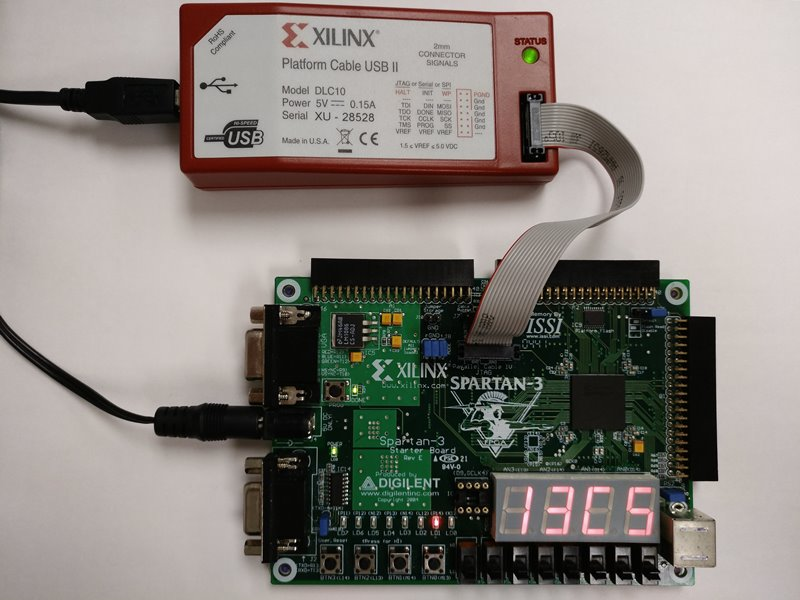
\includegraphics[width = 0.3\textwidth ]{CasoUso/10.jpg}  &
		 \includegraphics[width = 0.3\textwidth ]{CasoUso/12.jpg}   &
		 \includegraphics[width = 0.3\textwidth ]{CasoUso/13.jpg}  \\ 
	\end{tabular}
	\end{table}
	\begin{itemize}
	    \item 10.  Una vez ha esperado dicho tiempo se carga en la memoria el siguiente dato, el piso tres al cual nos dirigiremos ahora. El guardado en la memoria dos pasa a la primera (que será el siguiente piso), una vez llegado al tercer piso nos dirigimos al segundo. Estos ya no se reflejan en los LEDs destinados a la memoria, si no que vemos que se ha marcado el cuarto piso al que se ha llamado.
	    \item 11.  Una vez ha llegado al tercer piso nos dirigimos al segundo. Estos ya no se reflejan en los LEDs destinados a la memoria, si no que vemos que se ha marcado el cuarto piso.
	    \item 12. Cuando llega al segundo piso se carga el cuarto y la memoria queda vacia.
	\end{itemize}
	
	\begin{table}[H]
	\centering
	\begin{tabular}{ccc}
		 \includegraphics[width = 0.3\textwidth ]{CasoUso/14.jpg}   &  &  \\
	\end{tabular}
	\end{table}
	
	\begin{itemize}
	    \item 13. Una vez ha llegado al cuarto piso el ascensor se para y la puerta se abre.
	\end{itemize} %importa el fichero PruebasYResultados.tex
    
    \begin{appendices}
    \newpage
    \section{Codificación Entradas-Salidas} \label{app:codEntSal}
    
        \begin{table}[H]
        \centering
			\begin{tabular}{|c|c|c|c|}
				\hline
				\rowcolor[rgb]{0.21,0.69,0.87}\multicolumn{4}{|c|}{  \textbf{ {Codificación Pisos}}} \\
				\hline \hline
				 & \textbf{  PisoVoy (pulsadores)  } & \textbf{  PisoEstoy (finalCarrera)  } & \textbf{  7 Segmentos  }  \\
				\hline
				Piso1 & 0001 & 0001 & Imagen \\
				\hline
				Piso2 & 0010 & 0010 & Imagen \\
				\hline
				Piso3 & 0100 & 0100 & Imagen \\
				\hline
				Piso4 & 1000 & 1000 & Imagen \\
				\hline
				 
			\end{tabular}
			\caption{ Codificación para los diferentes pisos y su traducción  al número de piso y al display de 7 segmentos }
			\label{tab:tabla1ApendiceA}
		\end{table}
		
		
        \begin{table}[H]
        \centering
			\begin{tabular}{|c|c|}
				\hline
				\rowcolor[rgb]{0.21,0.69,0.87}\multicolumn{2}{|c|}{  \textbf{ {Funcionamiento Motor}}} \\
				\hline \hline
				 & \textbf{ Codificación Interna }  \\
				\hline
				Motor Parado & 00  \\
				\hline
				Motor girando en sentido de Subida & 01  \\
				\hline
				Motor girando en sentido de Bajada & 10 \\ 
				\hline
				 
			\end{tabular}
			\caption{ Codificación para los diferentes pisos y su traducción  al número de piso y al display de 7 segmentos }
			\label{tab:tabla2ApendiceA}
		\end{table}
		
		\begin{table}[H]
        \centering
			\begin{tabular}{|c|c|}
				\hline
				\rowcolor[rgb]{0.21,0.69,0.87}\multicolumn{2}{|c|}{  \textbf{ {Funcionamiento Puerta}}} \\
				\hline \hline
				 & \textbf{ Codificación Interna }  \\
				\hline
				Abierta & 0  \\
				\hline
				Cerrada & 1  \\
				\hline
				 
			\end{tabular}
			\caption{ Codificación para los diferentes pisos y su traducción  al número de piso y al display de 7 segmentos }
			\label{tab:tabla2ApendiceA}
		\end{table}
		
	\section{Codificación para display de 7 segmentos}	\label{app:7segmentos}
		\begin{table}[H]
        \centering
			\begin{tabular}{|ccccc|}
				\hline
				\rowcolor[rgb]{0.21,0.69,0.87}\multicolumn{5}{|c|}{  \textbf{ {Caracteres en binario para display de 7 segmentos}}} \\
				\hline \hline
				\multicolumn{3}{|c|}{  \textbf{ {Funcionamiento Motor}}} & \multicolumn{2}{|c|}{\textbf{Funcionamiento Puerta}} \\
				\hline
				 \includegraphics[width = 0.15\textwidth ]{CodCaracteres7s/subida} &
				 \includegraphics[width = 0.15\textwidth ]{CodCaracteres7s/bajada}  &
				 \includegraphics[width = 0.15\textwidth ]{CodCaracteres7s/parado} &
				 \includegraphics[width = 0.15\textwidth ]{CodCaracteres7s/cerrada}  &
				 \includegraphics[width = 0.15\textwidth ]{CodCaracteres7s/abierta}  \\
				 1011011 & 1111111 & 0000001 & 1001110 & 1110111 \\ 	
				\hline
				 \multicolumn{5}{|c|}{ \includegraphics[width = 1\textwidth ]{displays7s} } \\
				 1001111 & 0010010 & 0000110 & 1001100 & 0110000 \\ 
				\hline
			\end{tabular}
			\caption{ Codificación en binario para mostrar la información en el display de 7 segmentos }
			\label{tab:tabla1ApendiceB}
		\end{table}
	\newpage	
\end{appendices} %importa el fichero Apendices.tex

    \newpage
    \addcontentsline{toc}{section}{Índice de figuras} % para que aparezca en el indice de contenidos
    \listoffigures
    \addcontentsline{toc}{section}{Índice de tablas} % para que aparezca en el indice de contenidos
	\listoftables
	
\end{document}
